\documentclass[12pt]{article}
\usepackage[T1]{fontenc}
\usepackage[utf8]{inputenc}
\usepackage[default]{sourcesanspro}
\usepackage[letterpaper,left=0.5in,right=0.5in,top=0.7in,bottom=0.7in,headheight=15pt,headsep=12pt,footskip=26pt]{geometry}
\usepackage{fancyhdr}
\usepackage{tikz}
\pagestyle{fancy}
\fancyhf{}
\fancyhead[L]{Week 10 / Bridges / Grades 2--3}
\fancyfoot[L]{Bellingham Math Circle / Week 10 / F10-M-v4}
\fancyfoot[R]{\thepage}
\renewcommand{\headrulewidth}{0.4pt}
\renewcommand{\footrulewidth}{0pt}
\setlength{\parindent}{0pt}
\setlength{\parskip}{0pt}
\raggedright
\raggedbottom
\hyphenpenalty=10000
\exhyphenpenalty=10000
\frenchspacing
\newcommand{\prob}[1]{\textbf{Problem #1:}\ }
\tikzset{
  bandout/.style={line width=1.6cm, draw=black!75, line cap=butt},
  bandfill/.style={line width=1.480cm, draw=black!9, line cap=butt},
  island/.style={fill=white, draw=black, line width=1.3pt},
  islandlabel/.style={font=\sffamily\Large},
  stroke/.style={line width=1.4pt, draw=black!50, line cap=round, line join=round},
}

\begin{document}


Put a counter on every bridge of a town before you walk it. A walk starts on an island and crosses bridges one after another. Each time it crosses a bridge, pick up that bridge's counter. A bridge with no counter cannot be crossed. Two islands can be joined by more than one bridge. In every town you can get from any island to any other.

\vspace{6mm}

\begin{minipage}{\linewidth}\raggedright
\prob{1}In each town, find a walk that picks up every counter, and write its islands in order, like A~B~C~A.

\vspace{5mm}\noindent 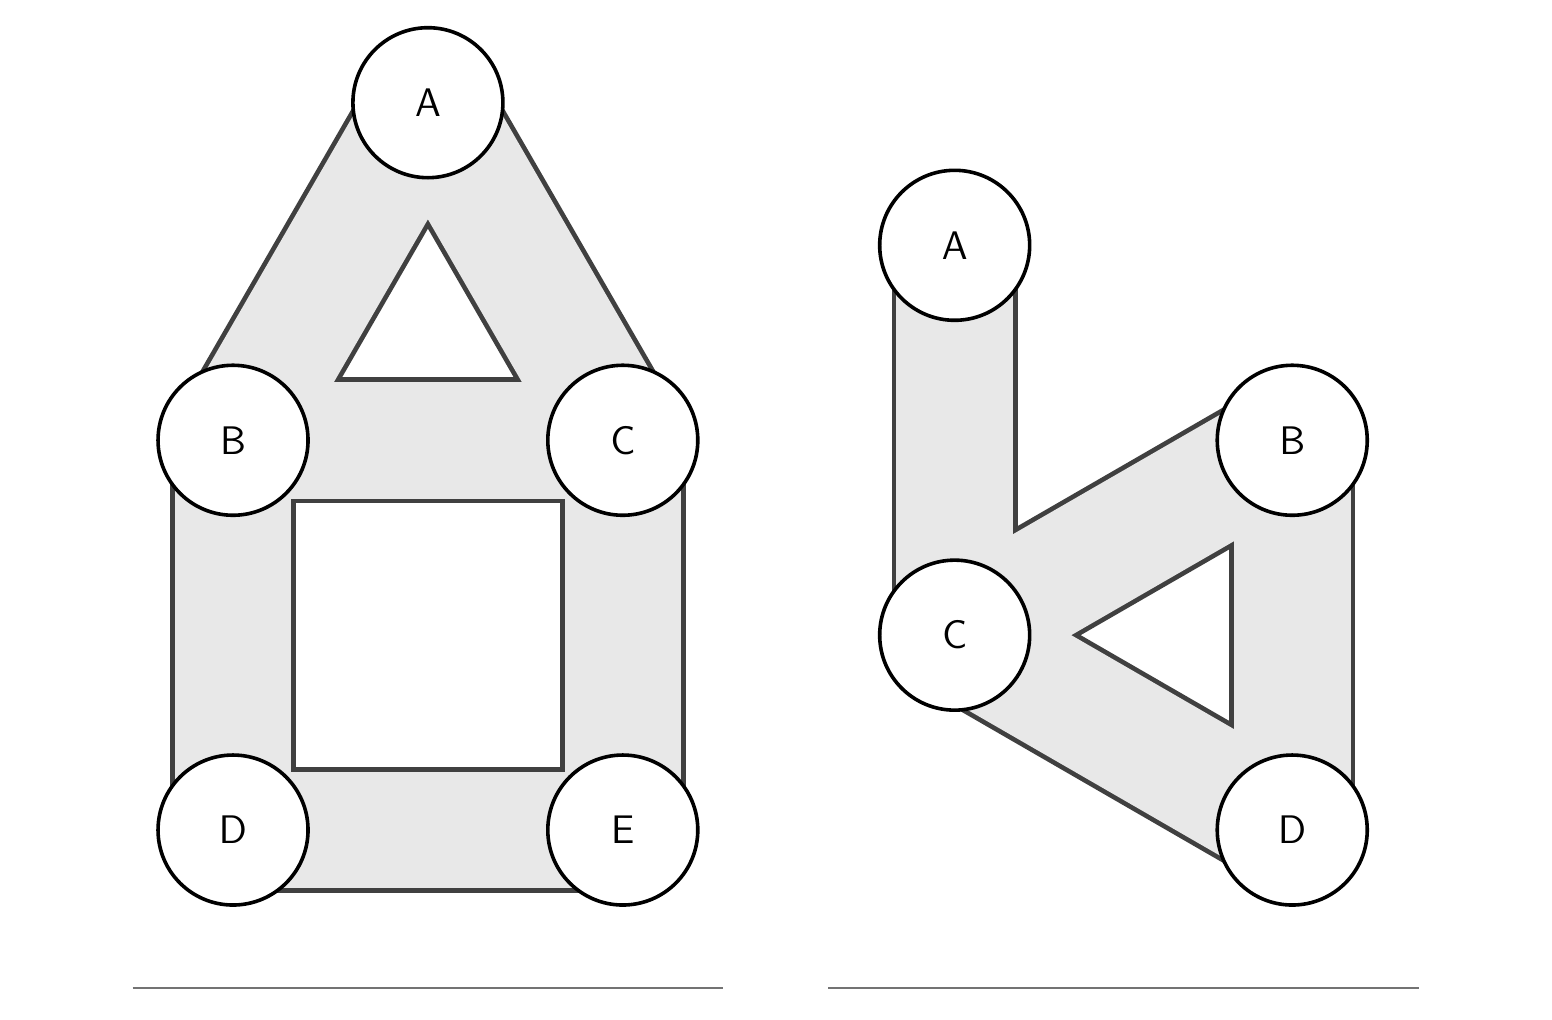
\begin{tikzpicture}
\useasboundingbox (0,0) rectangle (19.0,12.242);
\draw[bandout] (2.608,2.052) -- (7.558,2.052);
\draw[bandout] (7.558,2.052) -- (7.558,7.002);
\draw[bandout] (7.558,7.002) -- (2.608,7.002);
\draw[bandout] (2.608,7.002) -- (2.608,2.052);
\draw[bandout] (2.608,7.002) -- (5.083,11.289);
\draw[bandout] (5.083,11.289) -- (7.558,7.002);
\draw[bandfill] (2.608,2.052) -- (7.558,2.052);
\draw[bandfill] (7.558,2.052) -- (7.558,7.002);
\draw[bandfill] (7.558,7.002) -- (2.608,7.002);
\draw[bandfill] (2.608,7.002) -- (2.608,2.052);
\draw[bandfill] (2.608,7.002) -- (5.083,11.289);
\draw[bandfill] (5.083,11.289) -- (7.558,7.002);
\draw[island] (2.608,2.052) circle (0.9525);
\node[islandlabel] at (2.608,2.052) {D};
\draw[island] (7.558,2.052) circle (0.9525);
\node[islandlabel] at (7.558,2.052) {E};
\draw[island] (7.558,7.002) circle (0.9525);
\node[islandlabel] at (7.558,7.002) {C};
\draw[island] (2.608,7.002) circle (0.9525);
\node[islandlabel] at (2.608,7.002) {B};
\draw[island] (5.083,11.289) circle (0.9525);
\node[islandlabel] at (5.083,11.289) {A};
\draw[black!55, line width=0.6pt] (1.333,0.050) -- ++(7.5,0);
\draw[bandout] (16.060,2.052) -- (16.060,7.002);
\draw[bandout] (16.060,7.002) -- (11.773,4.527);
\draw[bandout] (11.773,4.527) -- (16.060,2.052);
\draw[bandout] (11.773,4.527) -- (11.773,9.478);
\draw[bandfill] (16.060,2.052) -- (16.060,7.002);
\draw[bandfill] (16.060,7.002) -- (11.773,4.527);
\draw[bandfill] (11.773,4.527) -- (16.060,2.052);
\draw[bandfill] (11.773,4.527) -- (11.773,9.478);
\draw[island] (16.060,2.052) circle (0.9525);
\node[islandlabel] at (16.060,2.052) {D};
\draw[island] (16.060,7.002) circle (0.9525);
\node[islandlabel] at (16.060,7.002) {B};
\draw[island] (11.773,4.527) circle (0.9525);
\node[islandlabel] at (11.773,4.527) {C};
\draw[island] (11.773,9.478) circle (0.9525);
\node[islandlabel] at (11.773,9.478) {A};
\draw[black!55, line width=0.6pt] (10.167,0.050) -- ++(7.5,0);
\end{tikzpicture}
\end{minipage}


\par\vspace{7mm}\noindent 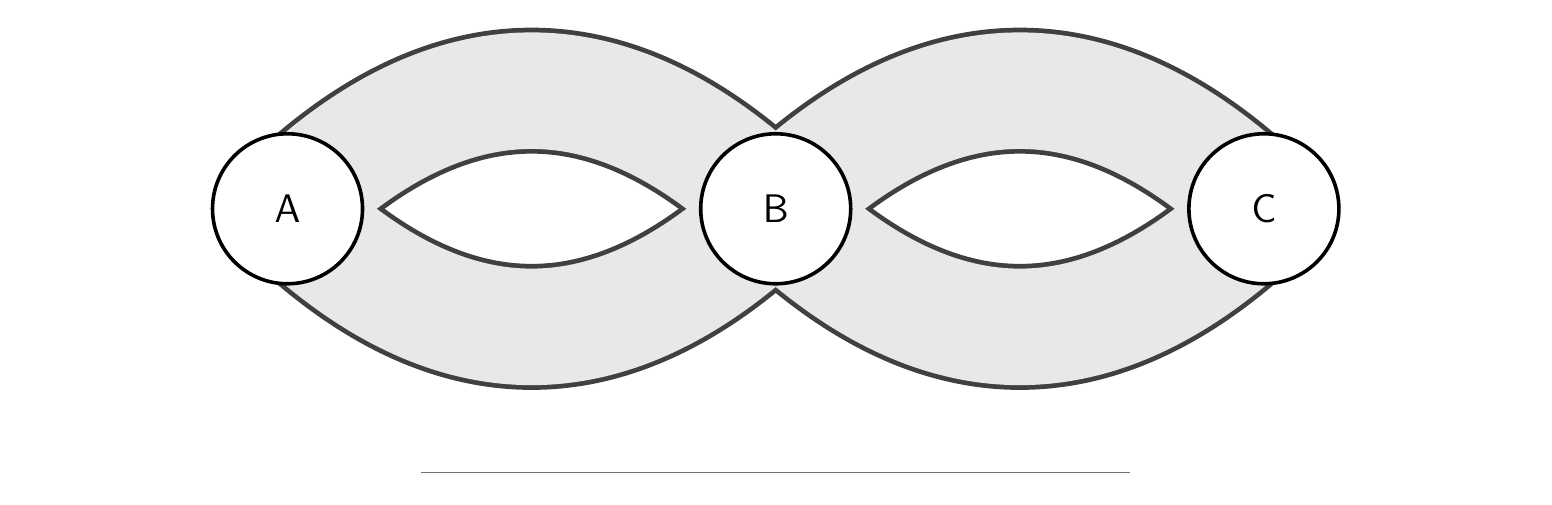
\begin{tikzpicture}
\useasboundingbox (0,0) rectangle (19.0,5.700);
\draw[bandout] (3.300,3.400) .. controls (5.367,5.400) and (7.433,5.400) .. (9.500,3.400);
\draw[bandout] (3.300,3.400) .. controls (5.367,1.400) and (7.433,1.400) .. (9.500,3.400);
\draw[bandout] (9.500,3.400) .. controls (11.567,5.400) and (13.633,5.400) .. (15.700,3.400);
\draw[bandout] (9.500,3.400) .. controls (11.567,1.400) and (13.633,1.400) .. (15.700,3.400);
\draw[bandfill] (3.300,3.400) .. controls (5.367,5.400) and (7.433,5.400) .. (9.500,3.400);
\draw[bandfill] (3.300,3.400) .. controls (5.367,1.400) and (7.433,1.400) .. (9.500,3.400);
\draw[bandfill] (9.500,3.400) .. controls (11.567,5.400) and (13.633,5.400) .. (15.700,3.400);
\draw[bandfill] (9.500,3.400) .. controls (11.567,1.400) and (13.633,1.400) .. (15.700,3.400);
\draw[island] (3.300,3.400) circle (0.9525);
\node[islandlabel] at (3.300,3.400) {A};
\draw[island] (9.500,3.400) circle (0.9525);
\node[islandlabel] at (9.500,3.400) {B};
\draw[island] (15.700,3.400) circle (0.9525);
\node[islandlabel] at (15.700,3.400) {C};
\draw[black!55, line width=0.6pt] (5.000,0.050) -- ++(9.0,0);
\end{tikzpicture}


\par\vspace{9mm}

\begin{minipage}{\linewidth}\raggedright
\prob{2}In each town, find every island where a walk that picks up every counter can start, and where such a walk can end. If a town has no such walk, write ``none''.

\vspace{5mm}\noindent 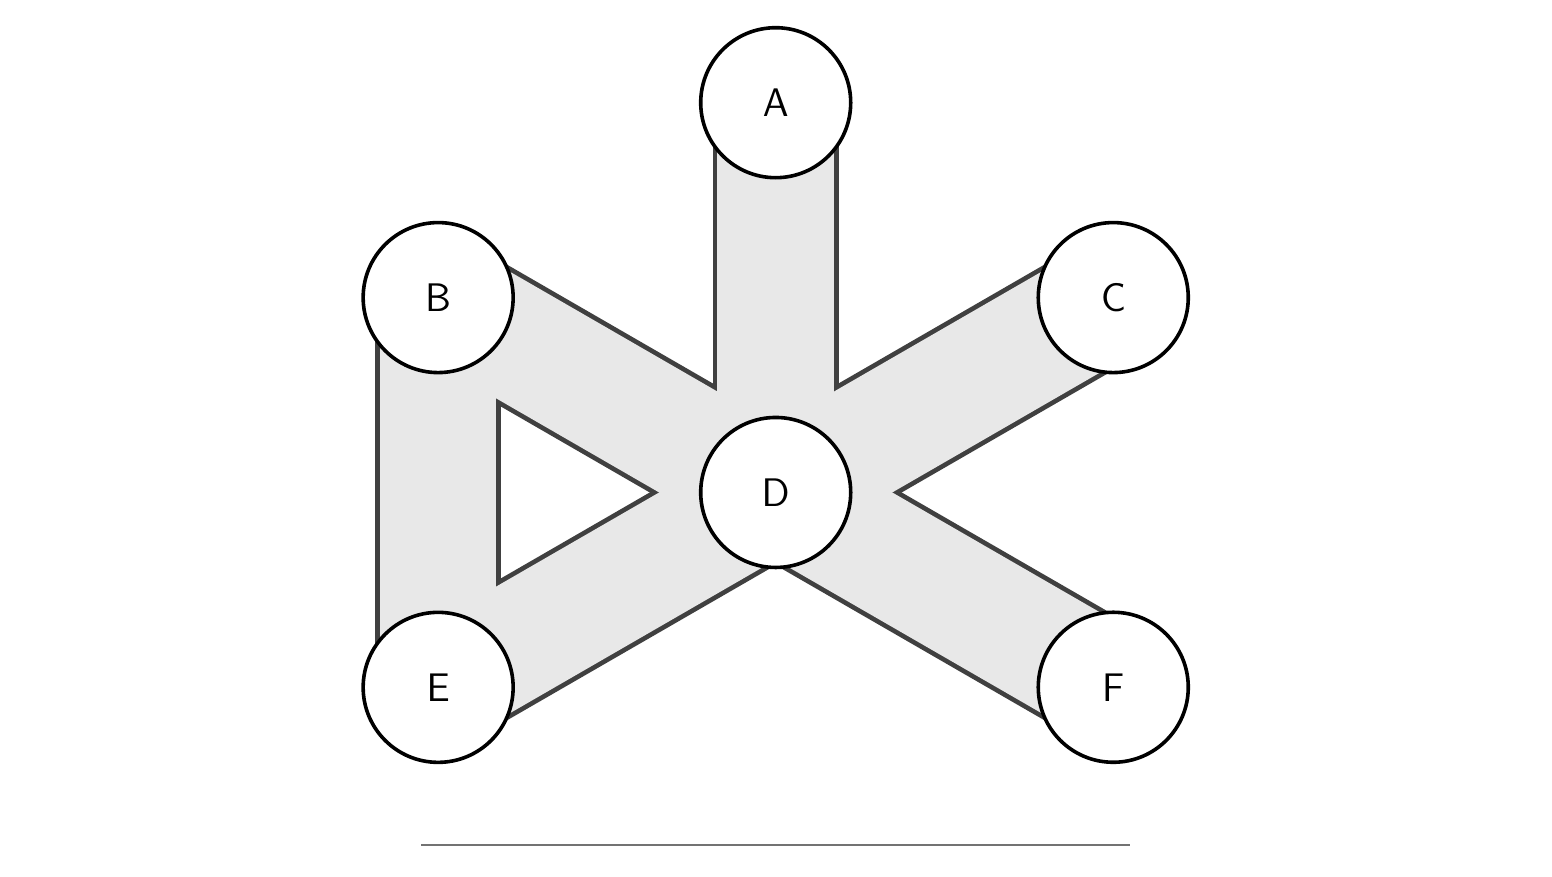
\begin{tikzpicture}
\useasboundingbox (0,0) rectangle (19.0,10.430);
\draw[bandout] (9.500,4.527) -- (5.213,2.052);
\draw[bandout] (9.500,4.527) -- (5.213,7.002);
\draw[bandout] (9.500,4.527) -- (13.787,7.002);
\draw[bandout] (9.500,4.527) -- (13.787,2.053);
\draw[bandout] (9.500,4.527) -- (9.500,9.477);
\draw[bandout] (5.213,2.052) -- (5.213,7.002);
\draw[bandfill] (9.500,4.527) -- (5.213,2.052);
\draw[bandfill] (9.500,4.527) -- (5.213,7.002);
\draw[bandfill] (9.500,4.527) -- (13.787,7.002);
\draw[bandfill] (9.500,4.527) -- (13.787,2.053);
\draw[bandfill] (9.500,4.527) -- (9.500,9.477);
\draw[bandfill] (5.213,2.052) -- (5.213,7.002);
\draw[island] (9.500,4.527) circle (0.9525);
\node[islandlabel] at (9.500,4.527) {D};
\draw[island] (5.213,2.052) circle (0.9525);
\node[islandlabel] at (5.213,2.052) {E};
\draw[island] (5.213,7.002) circle (0.9525);
\node[islandlabel] at (5.213,7.002) {B};
\draw[island] (13.787,7.002) circle (0.9525);
\node[islandlabel] at (13.787,7.002) {C};
\draw[island] (13.787,2.053) circle (0.9525);
\node[islandlabel] at (13.787,2.053) {F};
\draw[island] (9.500,9.477) circle (0.9525);
\node[islandlabel] at (9.500,9.477) {A};
\draw[black!55, line width=0.6pt] (5.000,0.050) -- ++(9.0,0);
\end{tikzpicture}
\end{minipage}


\par\vspace{7mm}\noindent 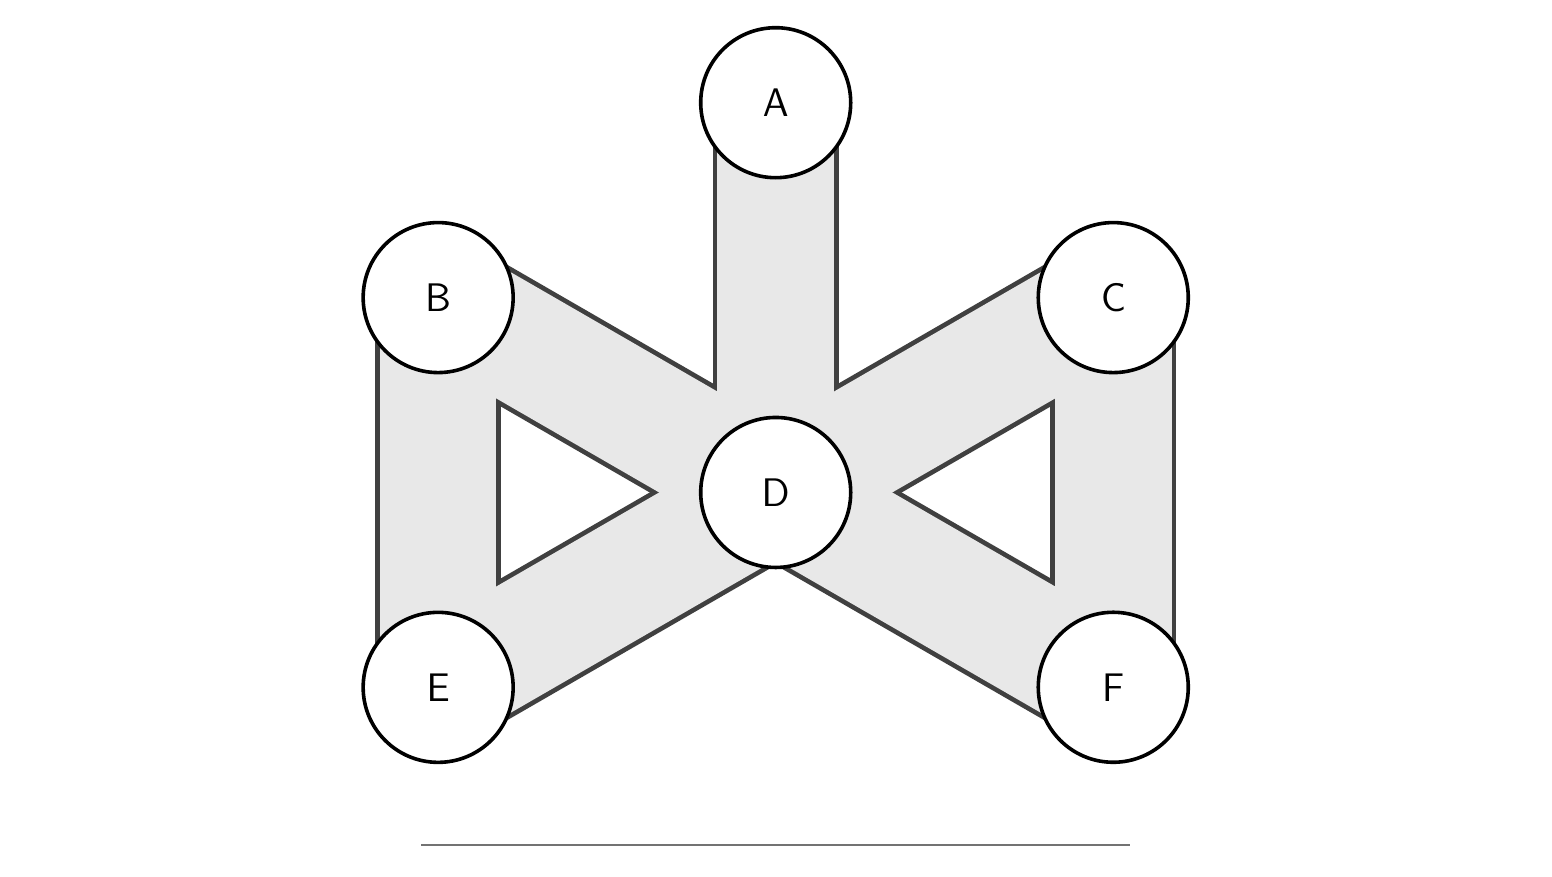
\begin{tikzpicture}
\useasboundingbox (0,0) rectangle (19.0,10.430);
\draw[bandout] (9.500,4.527) -- (5.213,2.052);
\draw[bandout] (9.500,4.527) -- (5.213,7.002);
\draw[bandout] (9.500,4.527) -- (13.787,7.002);
\draw[bandout] (9.500,4.527) -- (13.787,2.053);
\draw[bandout] (9.500,4.527) -- (9.500,9.477);
\draw[bandout] (5.213,2.052) -- (5.213,7.002);
\draw[bandout] (13.787,7.002) -- (13.787,2.053);
\draw[bandfill] (9.500,4.527) -- (5.213,2.052);
\draw[bandfill] (9.500,4.527) -- (5.213,7.002);
\draw[bandfill] (9.500,4.527) -- (13.787,7.002);
\draw[bandfill] (9.500,4.527) -- (13.787,2.053);
\draw[bandfill] (9.500,4.527) -- (9.500,9.477);
\draw[bandfill] (5.213,2.052) -- (5.213,7.002);
\draw[bandfill] (13.787,7.002) -- (13.787,2.053);
\draw[island] (9.500,4.527) circle (0.9525);
\node[islandlabel] at (9.500,4.527) {D};
\draw[island] (5.213,2.052) circle (0.9525);
\node[islandlabel] at (5.213,2.052) {E};
\draw[island] (5.213,7.002) circle (0.9525);
\node[islandlabel] at (5.213,7.002) {B};
\draw[island] (13.787,7.002) circle (0.9525);
\node[islandlabel] at (13.787,7.002) {C};
\draw[island] (13.787,2.053) circle (0.9525);
\node[islandlabel] at (13.787,2.053) {F};
\draw[island] (9.500,9.477) circle (0.9525);
\node[islandlabel] at (9.500,9.477) {A};
\draw[black!55, line width=0.6pt] (5.000,0.050) -- ++(9.0,0);
\end{tikzpicture}


\par\vspace{7mm}\noindent 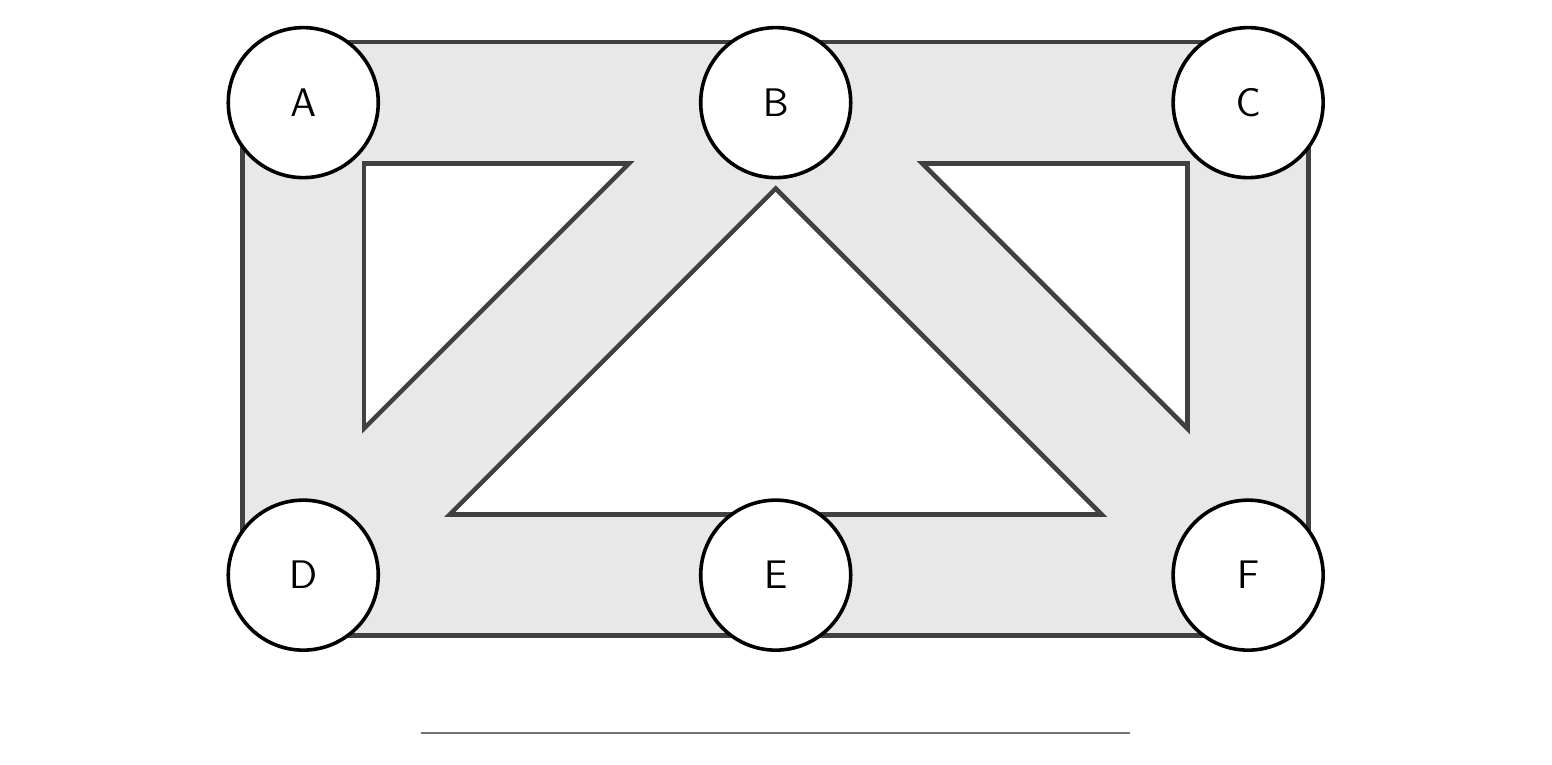
\begin{tikzpicture}
\useasboundingbox (0,0) rectangle (19.0,9.005);
\draw[bandout] (3.500,2.052) -- (9.500,2.052);
\draw[bandout] (9.500,2.052) -- (15.500,2.052);
\draw[bandout] (3.500,8.053) -- (9.500,8.053);
\draw[bandout] (9.500,8.053) -- (15.500,8.053);
\draw[bandout] (3.500,2.052) -- (3.500,8.053);
\draw[bandout] (15.500,2.052) -- (15.500,8.053);
\draw[bandout] (9.500,8.053) -- (3.500,2.052);
\draw[bandout] (9.500,8.053) -- (15.500,2.052);
\draw[bandfill] (3.500,2.052) -- (9.500,2.052);
\draw[bandfill] (9.500,2.052) -- (15.500,2.052);
\draw[bandfill] (3.500,8.053) -- (9.500,8.053);
\draw[bandfill] (9.500,8.053) -- (15.500,8.053);
\draw[bandfill] (3.500,2.052) -- (3.500,8.053);
\draw[bandfill] (15.500,2.052) -- (15.500,8.053);
\draw[bandfill] (9.500,8.053) -- (3.500,2.052);
\draw[bandfill] (9.500,8.053) -- (15.500,2.052);
\draw[island] (3.500,2.052) circle (0.9525);
\node[islandlabel] at (3.500,2.052) {D};
\draw[island] (3.500,8.053) circle (0.9525);
\node[islandlabel] at (3.500,8.053) {A};
\draw[island] (9.500,2.052) circle (0.9525);
\node[islandlabel] at (9.500,2.052) {E};
\draw[island] (9.500,8.053) circle (0.9525);
\node[islandlabel] at (9.500,8.053) {B};
\draw[island] (15.500,2.052) circle (0.9525);
\node[islandlabel] at (15.500,2.052) {F};
\draw[island] (15.500,8.053) circle (0.9525);
\node[islandlabel] at (15.500,8.053) {C};
\draw[black!55, line width=0.6pt] (5.000,0.050) -- ++(9.0,0);
\end{tikzpicture}


\par\vspace{7mm}\noindent 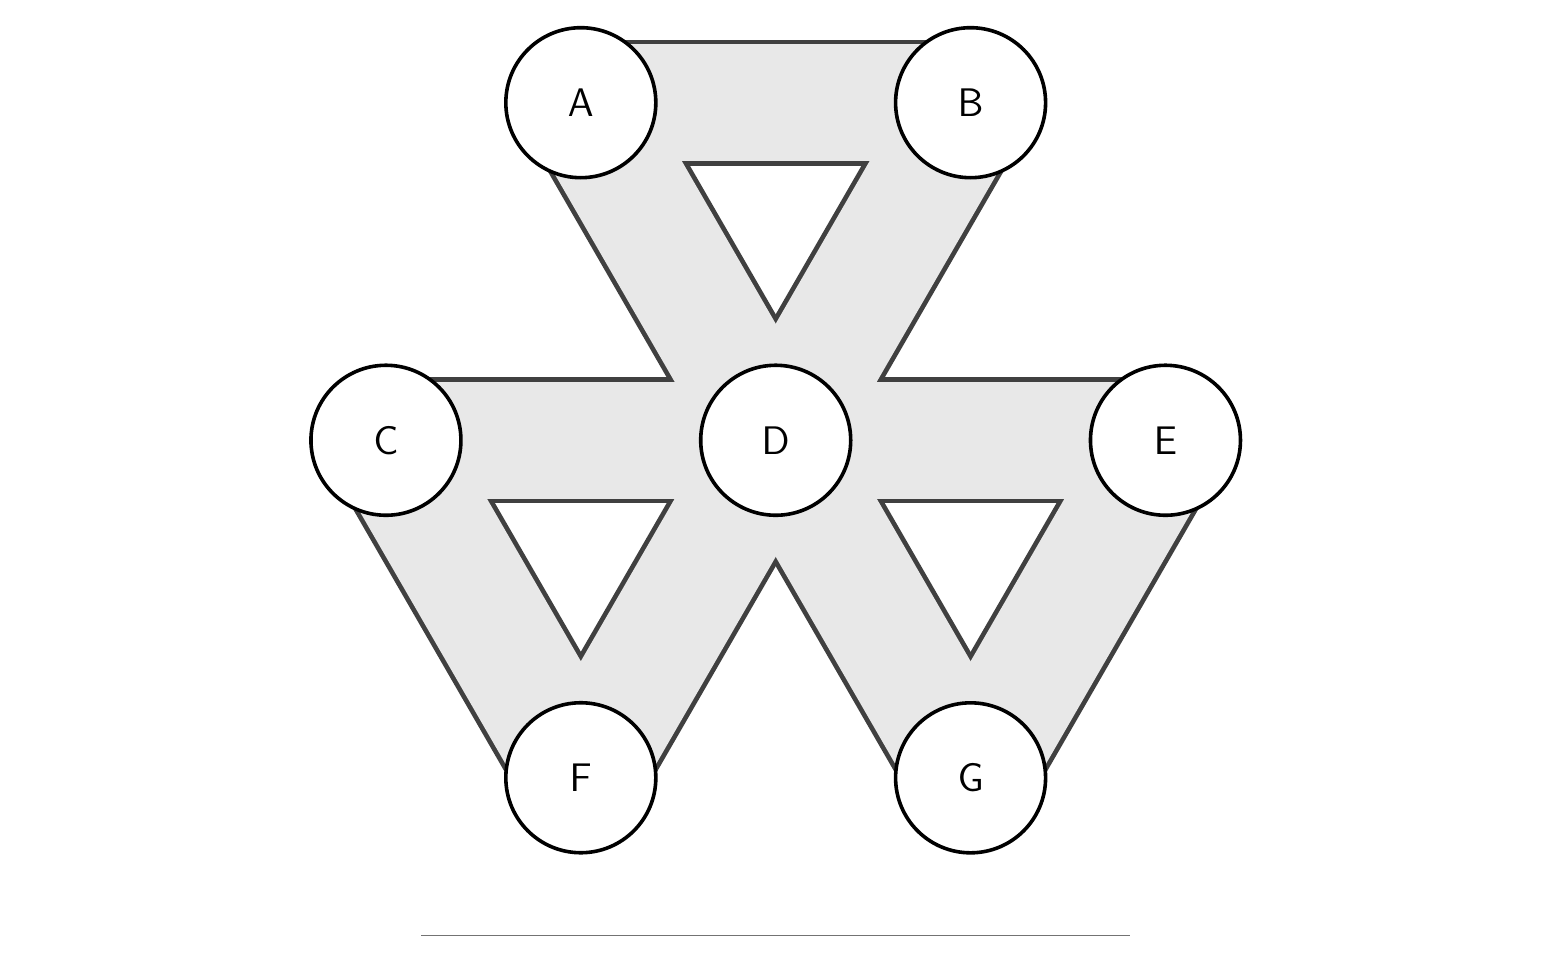
\begin{tikzpicture}
\useasboundingbox (0,0) rectangle (19.0,11.579);
\draw[bandout] (9.500,6.339) -- (11.975,10.626);
\draw[bandout] (11.975,10.626) -- (7.025,10.626);
\draw[bandout] (7.025,10.626) -- (9.500,6.339);
\draw[bandout] (9.500,6.339) -- (4.550,6.339);
\draw[bandout] (4.550,6.339) -- (7.025,2.053);
\draw[bandout] (7.025,2.053) -- (9.500,6.339);
\draw[bandout] (9.500,6.339) -- (11.975,2.052);
\draw[bandout] (11.975,2.052) -- (14.450,6.339);
\draw[bandout] (14.450,6.339) -- (9.500,6.339);
\draw[bandfill] (9.500,6.339) -- (11.975,10.626);
\draw[bandfill] (11.975,10.626) -- (7.025,10.626);
\draw[bandfill] (7.025,10.626) -- (9.500,6.339);
\draw[bandfill] (9.500,6.339) -- (4.550,6.339);
\draw[bandfill] (4.550,6.339) -- (7.025,2.053);
\draw[bandfill] (7.025,2.053) -- (9.500,6.339);
\draw[bandfill] (9.500,6.339) -- (11.975,2.052);
\draw[bandfill] (11.975,2.052) -- (14.450,6.339);
\draw[bandfill] (14.450,6.339) -- (9.500,6.339);
\draw[island] (9.500,6.339) circle (0.9525);
\node[islandlabel] at (9.500,6.339) {D};
\draw[island] (11.975,10.626) circle (0.9525);
\node[islandlabel] at (11.975,10.626) {B};
\draw[island] (7.025,10.626) circle (0.9525);
\node[islandlabel] at (7.025,10.626) {A};
\draw[island] (4.550,6.339) circle (0.9525);
\node[islandlabel] at (4.550,6.339) {C};
\draw[island] (7.025,2.053) circle (0.9525);
\node[islandlabel] at (7.025,2.053) {F};
\draw[island] (11.975,2.052) circle (0.9525);
\node[islandlabel] at (11.975,2.052) {G};
\draw[island] (14.450,6.339) circle (0.9525);
\node[islandlabel] at (14.450,6.339) {E};
\draw[black!55, line width=0.6pt] (5.000,0.050) -- ++(9.0,0);
\end{tikzpicture}


\par\vspace{9mm}

\begin{minipage}{\linewidth}\raggedright
\prob{3}For each town, decide without walking whether a walk can pick up every counter. If it can, circle every island where such a walk can start. If it cannot, write ``none''. Then check with counters.

\vspace{5mm}\noindent 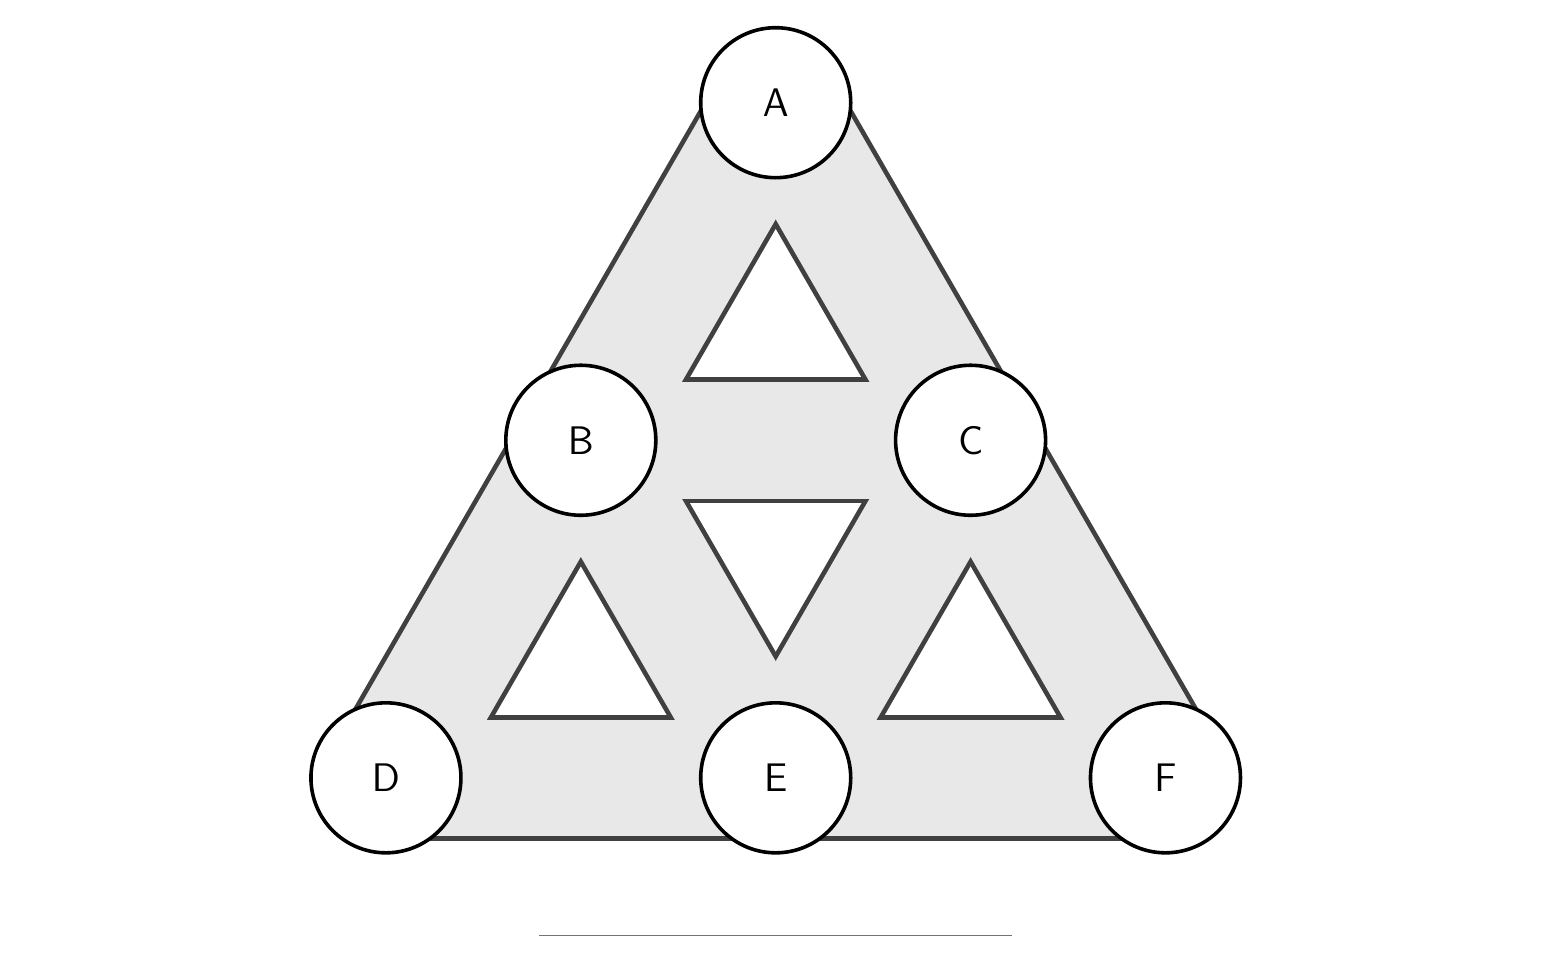
\begin{tikzpicture}
\useasboundingbox (0,0) rectangle (19.0,11.579);
\draw[bandout] (4.550,2.052) -- (9.500,2.052);
\draw[bandout] (9.500,2.052) -- (14.450,2.052);
\draw[bandout] (14.450,2.052) -- (11.975,6.339);
\draw[bandout] (11.975,6.339) -- (9.500,10.626);
\draw[bandout] (9.500,10.626) -- (7.025,6.339);
\draw[bandout] (7.025,6.339) -- (4.550,2.052);
\draw[bandout] (9.500,2.052) -- (11.975,6.339);
\draw[bandout] (11.975,6.339) -- (7.025,6.339);
\draw[bandout] (7.025,6.339) -- (9.500,2.052);
\draw[bandfill] (4.550,2.052) -- (9.500,2.052);
\draw[bandfill] (9.500,2.052) -- (14.450,2.052);
\draw[bandfill] (14.450,2.052) -- (11.975,6.339);
\draw[bandfill] (11.975,6.339) -- (9.500,10.626);
\draw[bandfill] (9.500,10.626) -- (7.025,6.339);
\draw[bandfill] (7.025,6.339) -- (4.550,2.052);
\draw[bandfill] (9.500,2.052) -- (11.975,6.339);
\draw[bandfill] (11.975,6.339) -- (7.025,6.339);
\draw[bandfill] (7.025,6.339) -- (9.500,2.052);
\draw[island] (4.550,2.052) circle (0.9525);
\node[islandlabel] at (4.550,2.052) {D};
\draw[island] (9.500,2.052) circle (0.9525);
\node[islandlabel] at (9.500,2.052) {E};
\draw[island] (14.450,2.052) circle (0.9525);
\node[islandlabel] at (14.450,2.052) {F};
\draw[island] (7.025,6.339) circle (0.9525);
\node[islandlabel] at (7.025,6.339) {B};
\draw[island] (11.975,6.339) circle (0.9525);
\node[islandlabel] at (11.975,6.339) {C};
\draw[island] (9.500,10.626) circle (0.9525);
\node[islandlabel] at (9.500,10.626) {A};
\draw[black!55, line width=0.6pt] (6.500,0.050) -- ++(6.0,0);
\end{tikzpicture}
\end{minipage}


\par\vspace{7mm}\noindent 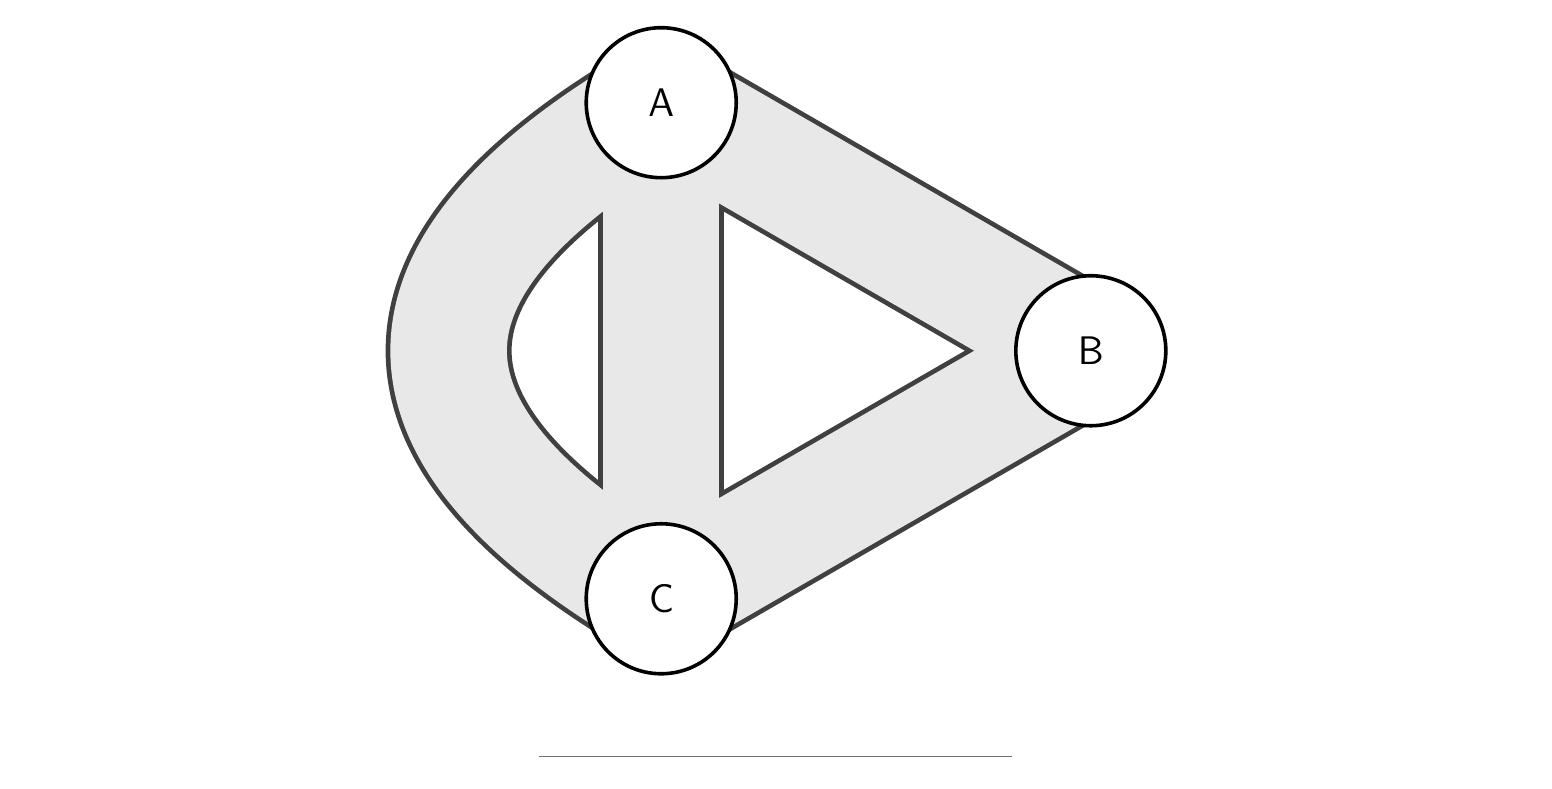
\begin{tikzpicture}
\useasboundingbox (0,0) rectangle (19.0,9.305);
\draw[bandout] (8.046,8.352) -- (8.046,2.052);
\draw[bandout] (8.046,8.352) .. controls (4.446,6.252) and (4.446,4.152) .. (8.046,2.052);
\draw[bandout] (8.046,8.352) -- (13.502,5.202);
\draw[bandout] (8.046,2.052) -- (13.502,5.202);
\draw[bandfill] (8.046,8.352) -- (8.046,2.052);
\draw[bandfill] (8.046,8.352) .. controls (4.446,6.252) and (4.446,4.152) .. (8.046,2.052);
\draw[bandfill] (8.046,8.352) -- (13.502,5.202);
\draw[bandfill] (8.046,2.052) -- (13.502,5.202);
\draw[island] (8.046,8.352) circle (0.9525);
\node[islandlabel] at (8.046,8.352) {A};
\draw[island] (8.046,2.052) circle (0.9525);
\node[islandlabel] at (8.046,2.052) {C};
\draw[island] (13.502,5.202) circle (0.9525);
\node[islandlabel] at (13.502,5.202) {B};
\draw[black!55, line width=0.6pt] (6.500,0.050) -- ++(6.0,0);
\end{tikzpicture}


\par\vspace{7mm}\noindent 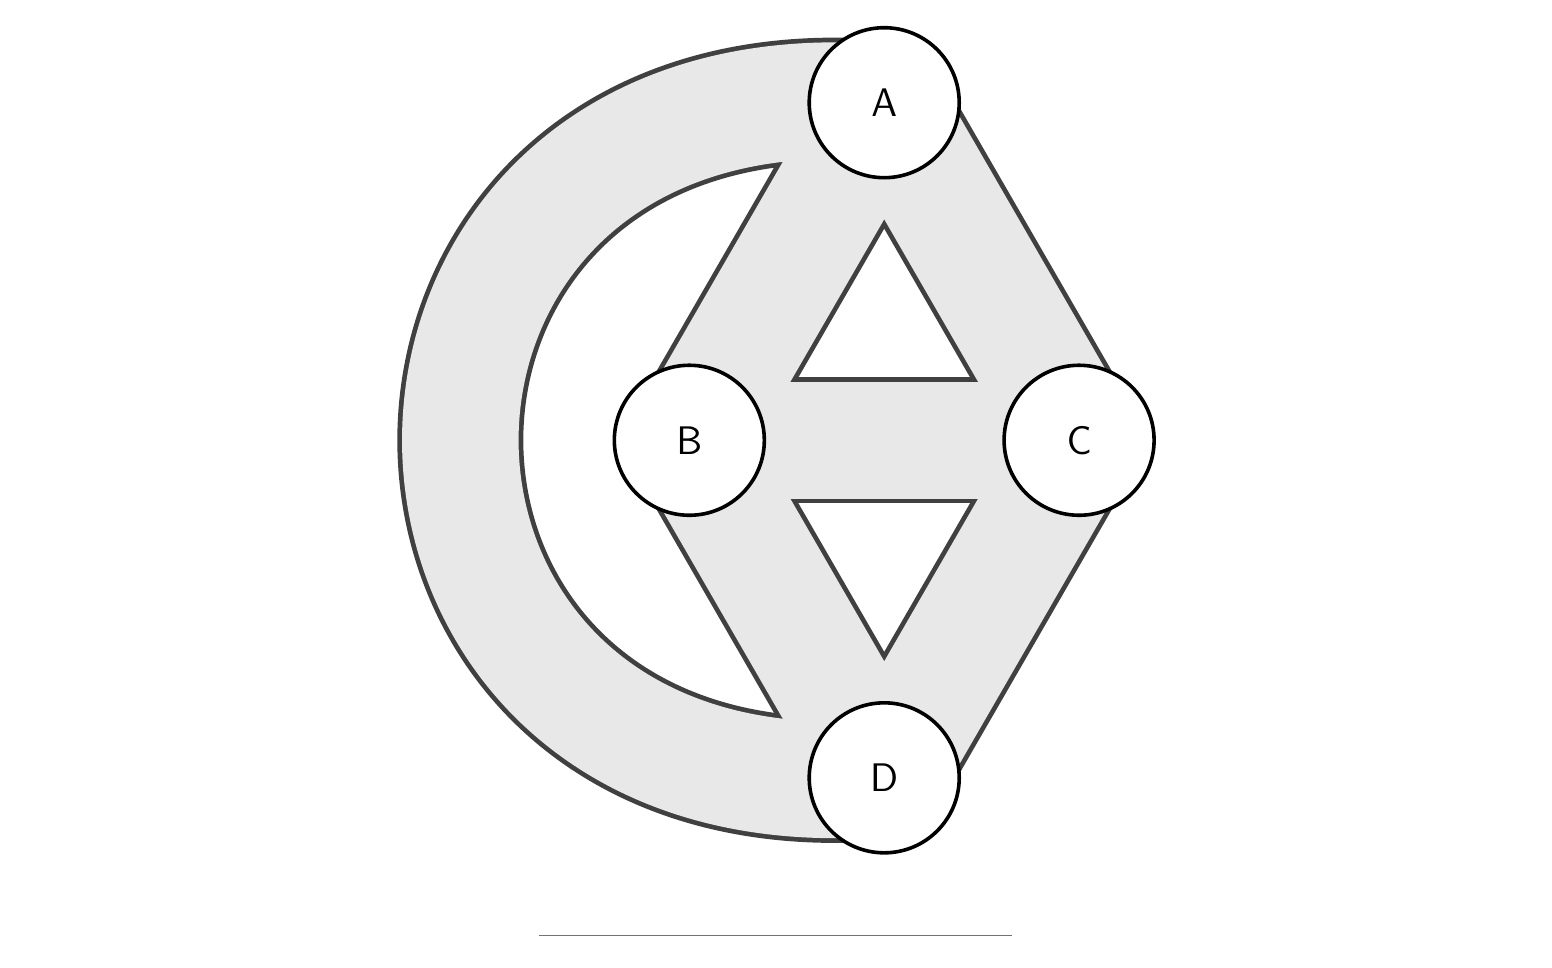
\begin{tikzpicture}
\useasboundingbox (0,0) rectangle (19.0,11.579);
\draw[bandout] (8.403,6.339) -- (13.353,6.339);
\draw[bandout] (8.403,6.339) -- (10.878,2.052);
\draw[bandout] (8.403,6.339) -- (10.878,10.626);
\draw[bandout] (13.353,6.339) -- (10.878,2.052);
\draw[bandout] (13.353,6.339) -- (10.878,10.626);
\draw[bandout] (10.878,2.052) .. controls (3.700,1.452) and (3.700,11.226) .. (10.878,10.626);
\draw[bandfill] (8.403,6.339) -- (13.353,6.339);
\draw[bandfill] (8.403,6.339) -- (10.878,2.052);
\draw[bandfill] (8.403,6.339) -- (10.878,10.626);
\draw[bandfill] (13.353,6.339) -- (10.878,2.052);
\draw[bandfill] (13.353,6.339) -- (10.878,10.626);
\draw[bandfill] (10.878,2.052) .. controls (3.700,1.452) and (3.700,11.226) .. (10.878,10.626);
\draw[island] (8.403,6.339) circle (0.9525);
\node[islandlabel] at (8.403,6.339) {B};
\draw[island] (13.353,6.339) circle (0.9525);
\node[islandlabel] at (13.353,6.339) {C};
\draw[island] (10.878,2.052) circle (0.9525);
\node[islandlabel] at (10.878,2.052) {D};
\draw[island] (10.878,10.626) circle (0.9525);
\node[islandlabel] at (10.878,10.626) {A};
\draw[black!55, line width=0.6pt] (6.500,0.050) -- ++(6.0,0);
\end{tikzpicture}


\par\vspace{7mm}\noindent 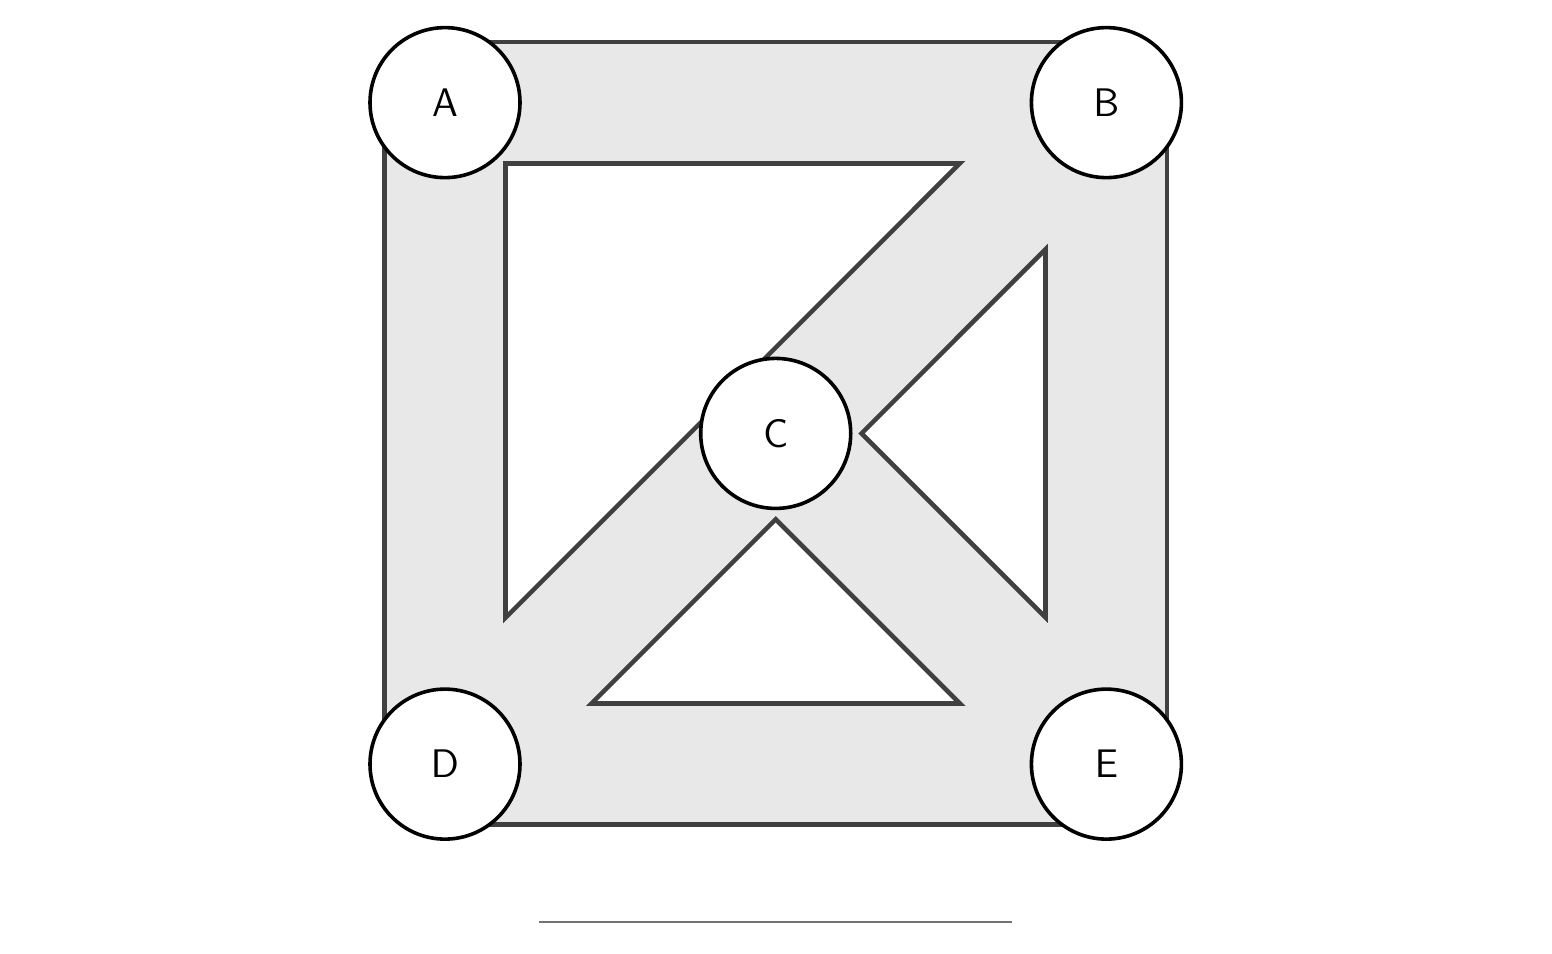
\begin{tikzpicture}
\useasboundingbox (0,0) rectangle (19.0,11.405);
\draw[bandout] (5.300,2.052) -- (13.700,2.052);
\draw[bandout] (13.700,2.052) -- (13.700,10.453);
\draw[bandout] (13.700,10.453) -- (5.300,10.453);
\draw[bandout] (5.300,10.453) -- (5.300,2.052);
\draw[bandout] (9.500,6.252) -- (5.300,2.052);
\draw[bandout] (9.500,6.252) -- (13.700,2.052);
\draw[bandout] (9.500,6.252) -- (13.700,10.453);
\draw[bandfill] (5.300,2.052) -- (13.700,2.052);
\draw[bandfill] (13.700,2.052) -- (13.700,10.453);
\draw[bandfill] (13.700,10.453) -- (5.300,10.453);
\draw[bandfill] (5.300,10.453) -- (5.300,2.052);
\draw[bandfill] (9.500,6.252) -- (5.300,2.052);
\draw[bandfill] (9.500,6.252) -- (13.700,2.052);
\draw[bandfill] (9.500,6.252) -- (13.700,10.453);
\draw[island] (5.300,2.052) circle (0.9525);
\node[islandlabel] at (5.300,2.052) {D};
\draw[island] (13.700,2.052) circle (0.9525);
\node[islandlabel] at (13.700,2.052) {E};
\draw[island] (13.700,10.453) circle (0.9525);
\node[islandlabel] at (13.700,10.453) {B};
\draw[island] (5.300,10.453) circle (0.9525);
\node[islandlabel] at (5.300,10.453) {A};
\draw[island] (9.500,6.252) circle (0.9525);
\node[islandlabel] at (9.500,6.252) {C};
\draw[black!55, line width=0.6pt] (6.500,0.050) -- ++(6.0,0);
\end{tikzpicture}


\par\vspace{9mm}

\begin{minipage}{\linewidth}\raggedright
\prob{4}No walk picks up every counter in these towns. In each town, draw one new bridge so that a walk can, and write the walk.

\vspace{5mm}\noindent 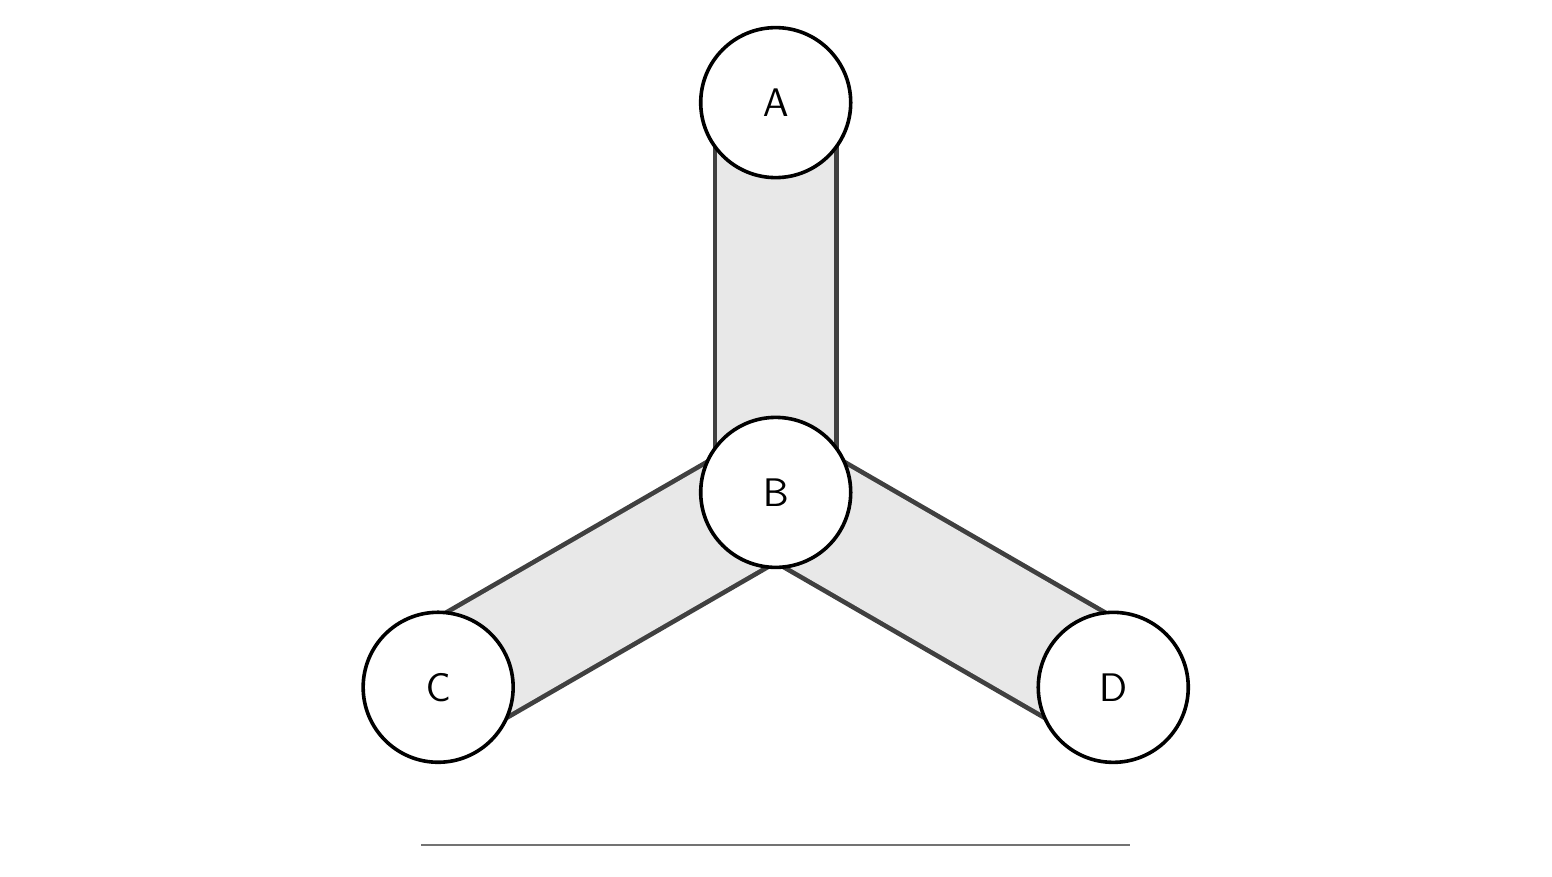
\begin{tikzpicture}
\useasboundingbox (0,0) rectangle (19.0,10.430);
\draw[bandout] (9.500,4.528) -- (9.500,9.478);
\draw[bandout] (9.500,4.528) -- (5.213,2.053);
\draw[bandout] (9.500,4.528) -- (13.787,2.052);
\draw[bandfill] (9.500,4.528) -- (9.500,9.478);
\draw[bandfill] (9.500,4.528) -- (5.213,2.053);
\draw[bandfill] (9.500,4.528) -- (13.787,2.052);
\draw[island] (9.500,4.528) circle (0.9525);
\node[islandlabel] at (9.500,4.528) {B};
\draw[island] (9.500,9.478) circle (0.9525);
\node[islandlabel] at (9.500,9.478) {A};
\draw[island] (5.213,2.053) circle (0.9525);
\node[islandlabel] at (5.213,2.053) {C};
\draw[island] (13.787,2.052) circle (0.9525);
\node[islandlabel] at (13.787,2.052) {D};
\draw[black!55, line width=0.6pt] (5.000,0.050) -- ++(9.0,0);
\end{tikzpicture}
\end{minipage}


\par\vspace{7mm}\noindent 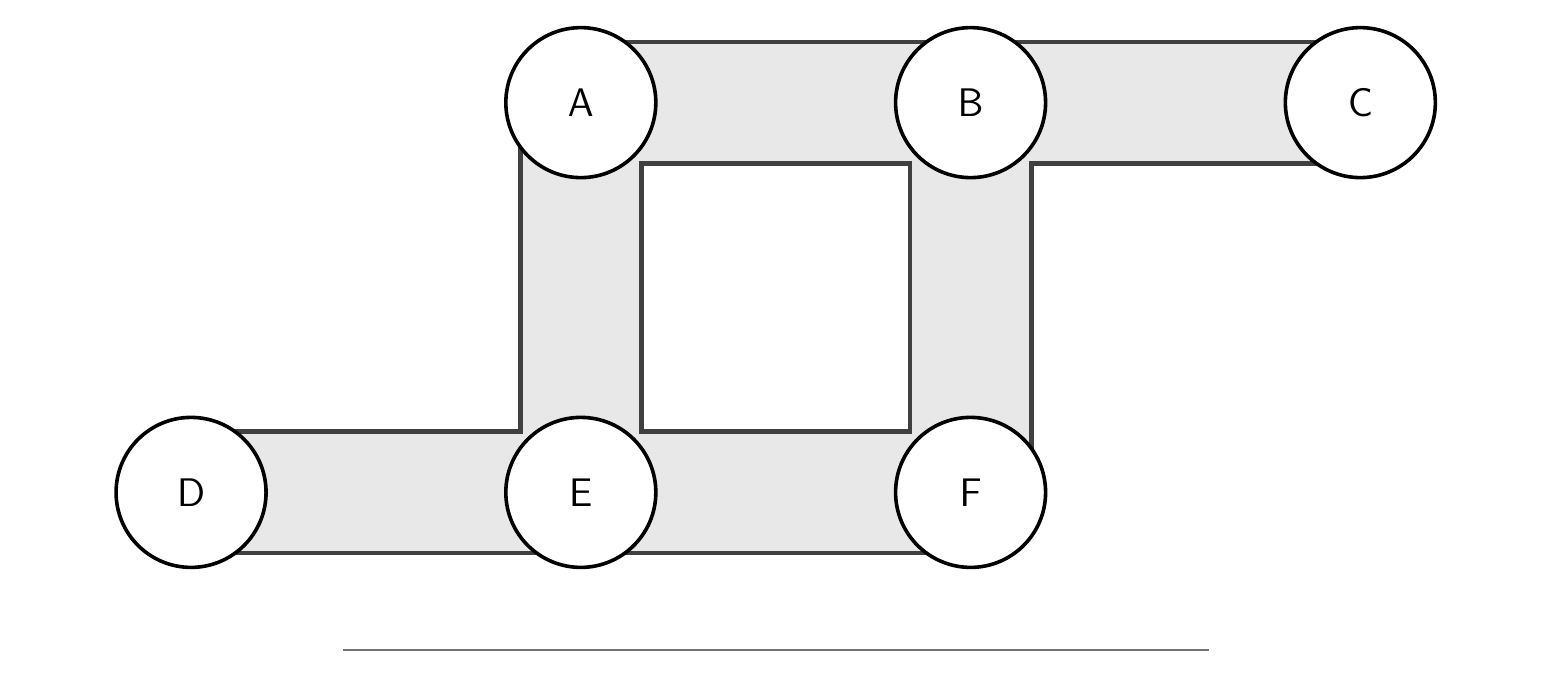
\begin{tikzpicture}
\useasboundingbox (0,0) rectangle (19.0,7.955);
\draw[bandout] (7.025,2.053) -- (11.975,2.053);
\draw[bandout] (11.975,2.053) -- (11.975,7.003);
\draw[bandout] (11.975,7.003) -- (7.025,7.003);
\draw[bandout] (7.025,7.003) -- (7.025,2.053);
\draw[bandout] (2.075,2.053) -- (7.025,2.053);
\draw[bandout] (11.975,7.003) -- (16.925,7.003);
\draw[bandfill] (7.025,2.053) -- (11.975,2.053);
\draw[bandfill] (11.975,2.053) -- (11.975,7.003);
\draw[bandfill] (11.975,7.003) -- (7.025,7.003);
\draw[bandfill] (7.025,7.003) -- (7.025,2.053);
\draw[bandfill] (2.075,2.053) -- (7.025,2.053);
\draw[bandfill] (11.975,7.003) -- (16.925,7.003);
\draw[island] (7.025,2.053) circle (0.9525);
\node[islandlabel] at (7.025,2.053) {E};
\draw[island] (11.975,2.053) circle (0.9525);
\node[islandlabel] at (11.975,2.053) {F};
\draw[island] (11.975,7.003) circle (0.9525);
\node[islandlabel] at (11.975,7.003) {B};
\draw[island] (7.025,7.003) circle (0.9525);
\node[islandlabel] at (7.025,7.003) {A};
\draw[island] (2.075,2.053) circle (0.9525);
\node[islandlabel] at (2.075,2.053) {D};
\draw[island] (16.925,7.003) circle (0.9525);
\node[islandlabel] at (16.925,7.003) {C};
\draw[black!55, line width=0.6pt] (4.000,0.050) -- ++(11.0,0);
\end{tikzpicture}


\par\vspace{7mm}\noindent 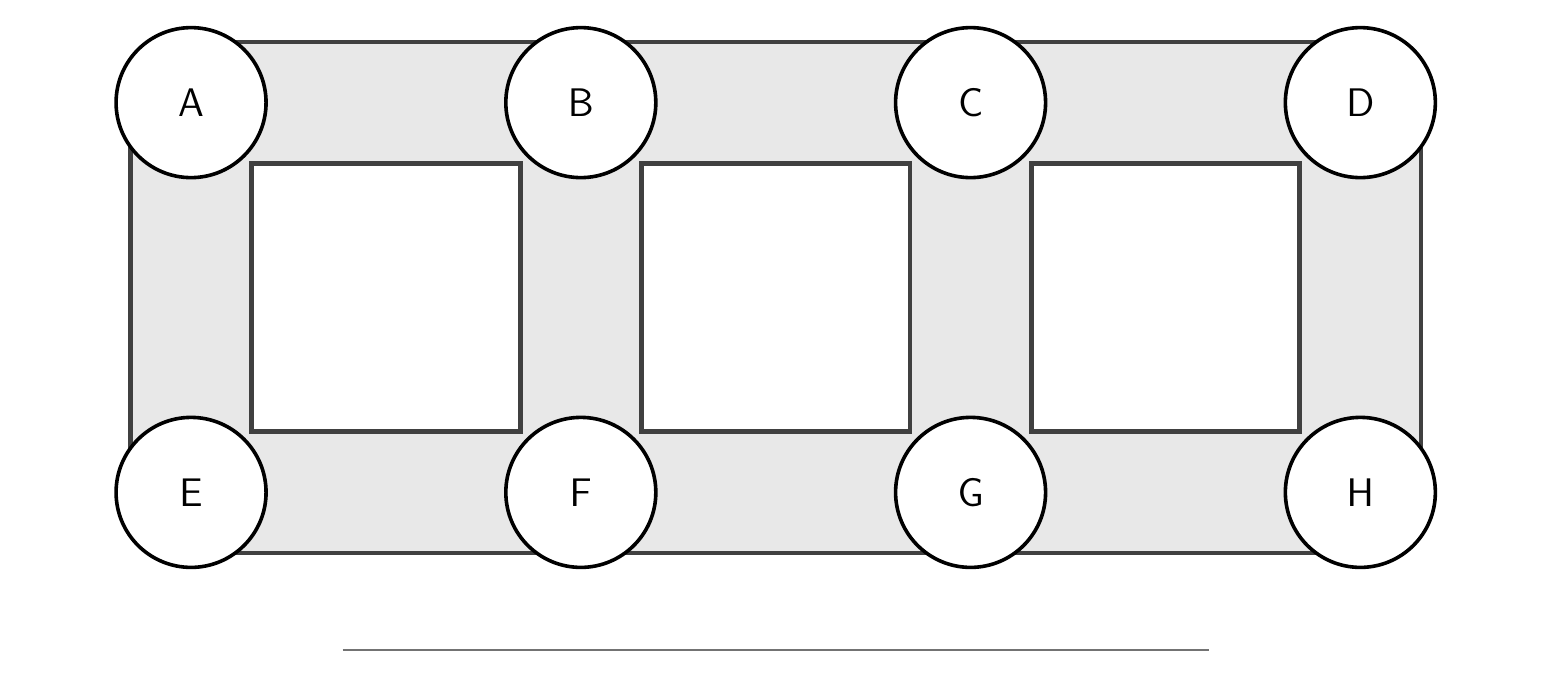
\begin{tikzpicture}
\useasboundingbox (0,0) rectangle (19.0,7.955);
\draw[bandout] (2.075,2.053) -- (7.025,2.053);
\draw[bandout] (2.075,7.003) -- (7.025,7.003);
\draw[bandout] (7.025,2.053) -- (11.975,2.053);
\draw[bandout] (7.025,7.003) -- (11.975,7.003);
\draw[bandout] (11.975,2.053) -- (16.925,2.053);
\draw[bandout] (11.975,7.003) -- (16.925,7.003);
\draw[bandout] (2.075,2.053) -- (2.075,7.003);
\draw[bandout] (7.025,2.053) -- (7.025,7.003);
\draw[bandout] (11.975,2.053) -- (11.975,7.003);
\draw[bandout] (16.925,2.053) -- (16.925,7.003);
\draw[bandfill] (2.075,2.053) -- (7.025,2.053);
\draw[bandfill] (2.075,7.003) -- (7.025,7.003);
\draw[bandfill] (7.025,2.053) -- (11.975,2.053);
\draw[bandfill] (7.025,7.003) -- (11.975,7.003);
\draw[bandfill] (11.975,2.053) -- (16.925,2.053);
\draw[bandfill] (11.975,7.003) -- (16.925,7.003);
\draw[bandfill] (2.075,2.053) -- (2.075,7.003);
\draw[bandfill] (7.025,2.053) -- (7.025,7.003);
\draw[bandfill] (11.975,2.053) -- (11.975,7.003);
\draw[bandfill] (16.925,2.053) -- (16.925,7.003);
\draw[island] (2.075,2.053) circle (0.9525);
\node[islandlabel] at (2.075,2.053) {E};
\draw[island] (7.025,2.053) circle (0.9525);
\node[islandlabel] at (7.025,2.053) {F};
\draw[island] (11.975,2.053) circle (0.9525);
\node[islandlabel] at (11.975,2.053) {G};
\draw[island] (16.925,2.053) circle (0.9525);
\node[islandlabel] at (16.925,2.053) {H};
\draw[island] (2.075,7.003) circle (0.9525);
\node[islandlabel] at (2.075,7.003) {A};
\draw[island] (7.025,7.003) circle (0.9525);
\node[islandlabel] at (7.025,7.003) {B};
\draw[island] (11.975,7.003) circle (0.9525);
\node[islandlabel] at (11.975,7.003) {C};
\draw[island] (16.925,7.003) circle (0.9525);
\node[islandlabel] at (16.925,7.003) {D};
\draw[black!55, line width=0.6pt] (4.000,0.050) -- ++(11.0,0);
\end{tikzpicture}


\par\vspace{9mm}

\begin{minipage}{\linewidth}\raggedright
\prob{5}In each town, draw as few new bridges as you can so that a walk can pick up every counter and end on the island where it started.

\vspace{5mm}\noindent 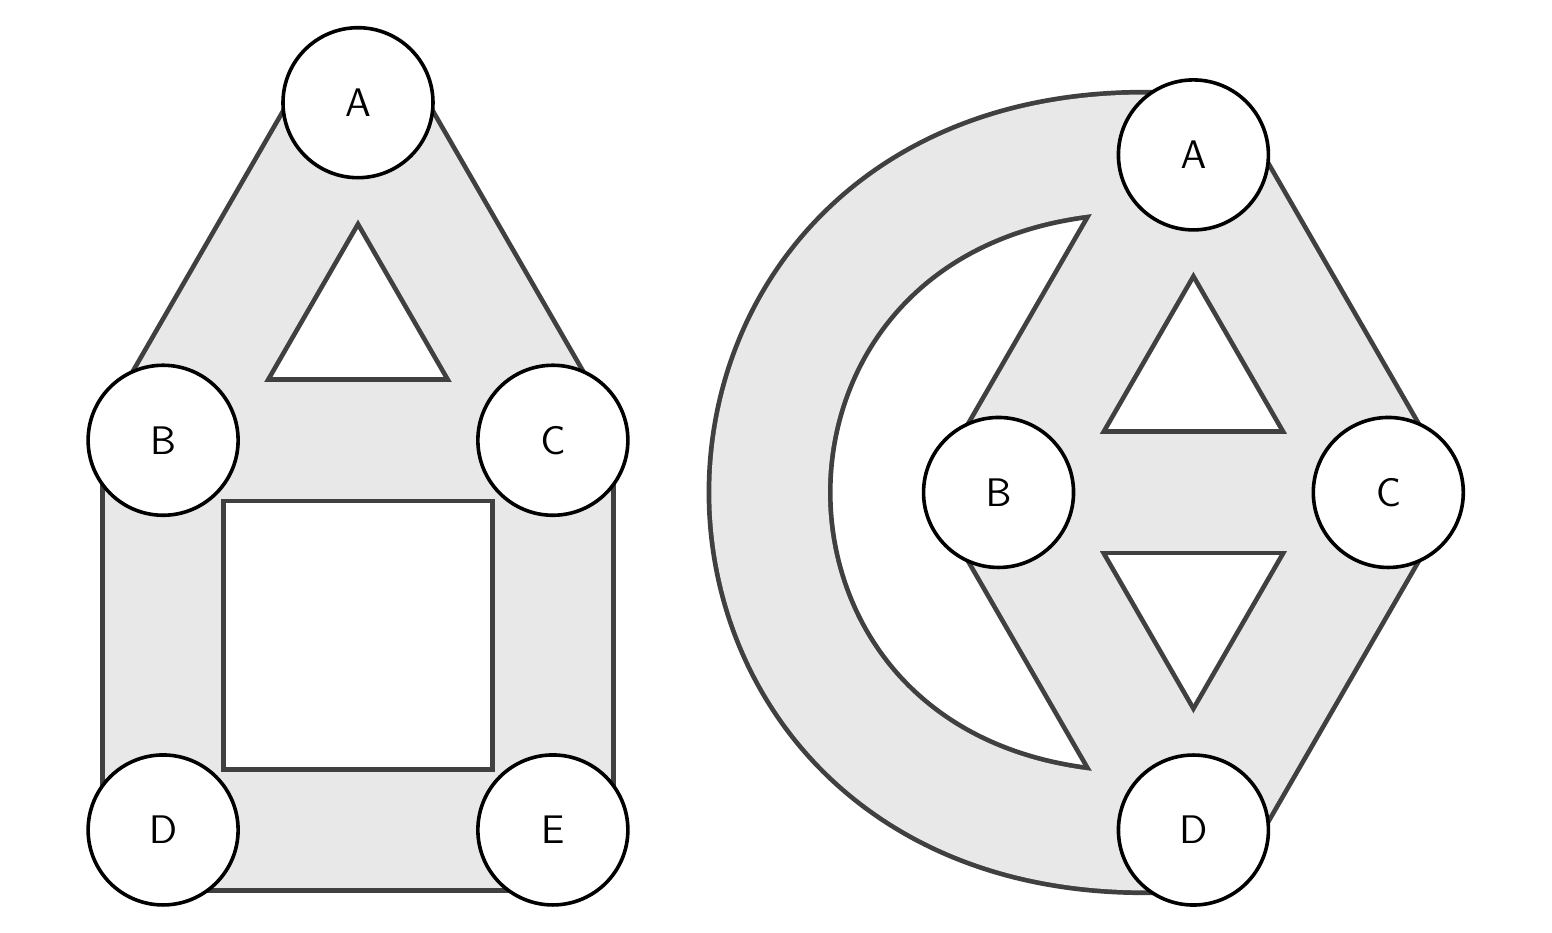
\begin{tikzpicture}
\useasboundingbox (0,0) rectangle (19.0,11.142);
\draw[bandout] (1.720,0.953) -- (6.670,0.953);
\draw[bandout] (6.670,0.953) -- (6.670,5.902);
\draw[bandout] (6.670,5.902) -- (1.720,5.902);
\draw[bandout] (1.720,5.902) -- (1.720,0.953);
\draw[bandout] (1.720,5.902) -- (4.195,10.189);
\draw[bandout] (4.195,10.189) -- (6.670,5.902);
\draw[bandfill] (1.720,0.953) -- (6.670,0.953);
\draw[bandfill] (6.670,0.953) -- (6.670,5.902);
\draw[bandfill] (6.670,5.902) -- (1.720,5.902);
\draw[bandfill] (1.720,5.902) -- (1.720,0.953);
\draw[bandfill] (1.720,5.902) -- (4.195,10.189);
\draw[bandfill] (4.195,10.189) -- (6.670,5.902);
\draw[island] (1.720,0.953) circle (0.9525);
\node[islandlabel] at (1.720,0.953) {D};
\draw[island] (6.670,0.953) circle (0.9525);
\node[islandlabel] at (6.670,0.953) {E};
\draw[island] (6.670,5.902) circle (0.9525);
\node[islandlabel] at (6.670,5.902) {C};
\draw[island] (1.720,5.902) circle (0.9525);
\node[islandlabel] at (1.720,5.902) {B};
\draw[island] (4.195,10.189) circle (0.9525);
\node[islandlabel] at (4.195,10.189) {A};
\draw[bandout] (12.330,5.239) -- (17.280,5.239);
\draw[bandout] (12.330,5.239) -- (14.805,0.952);
\draw[bandout] (12.330,5.239) -- (14.805,9.526);
\draw[bandout] (17.280,5.239) -- (14.805,0.952);
\draw[bandout] (17.280,5.239) -- (14.805,9.526);
\draw[bandout] (14.805,0.952) .. controls (7.628,0.353) and (7.628,10.126) .. (14.805,9.526);
\draw[bandfill] (12.330,5.239) -- (17.280,5.239);
\draw[bandfill] (12.330,5.239) -- (14.805,0.952);
\draw[bandfill] (12.330,5.239) -- (14.805,9.526);
\draw[bandfill] (17.280,5.239) -- (14.805,0.952);
\draw[bandfill] (17.280,5.239) -- (14.805,9.526);
\draw[bandfill] (14.805,0.952) .. controls (7.628,0.353) and (7.628,10.126) .. (14.805,9.526);
\draw[island] (12.330,5.239) circle (0.9525);
\node[islandlabel] at (12.330,5.239) {B};
\draw[island] (17.280,5.239) circle (0.9525);
\node[islandlabel] at (17.280,5.239) {C};
\draw[island] (14.805,0.952) circle (0.9525);
\node[islandlabel] at (14.805,0.952) {D};
\draw[island] (14.805,9.526) circle (0.9525);
\node[islandlabel] at (14.805,9.526) {A};
\end{tikzpicture}
\end{minipage}


\par\vspace{7mm}\noindent 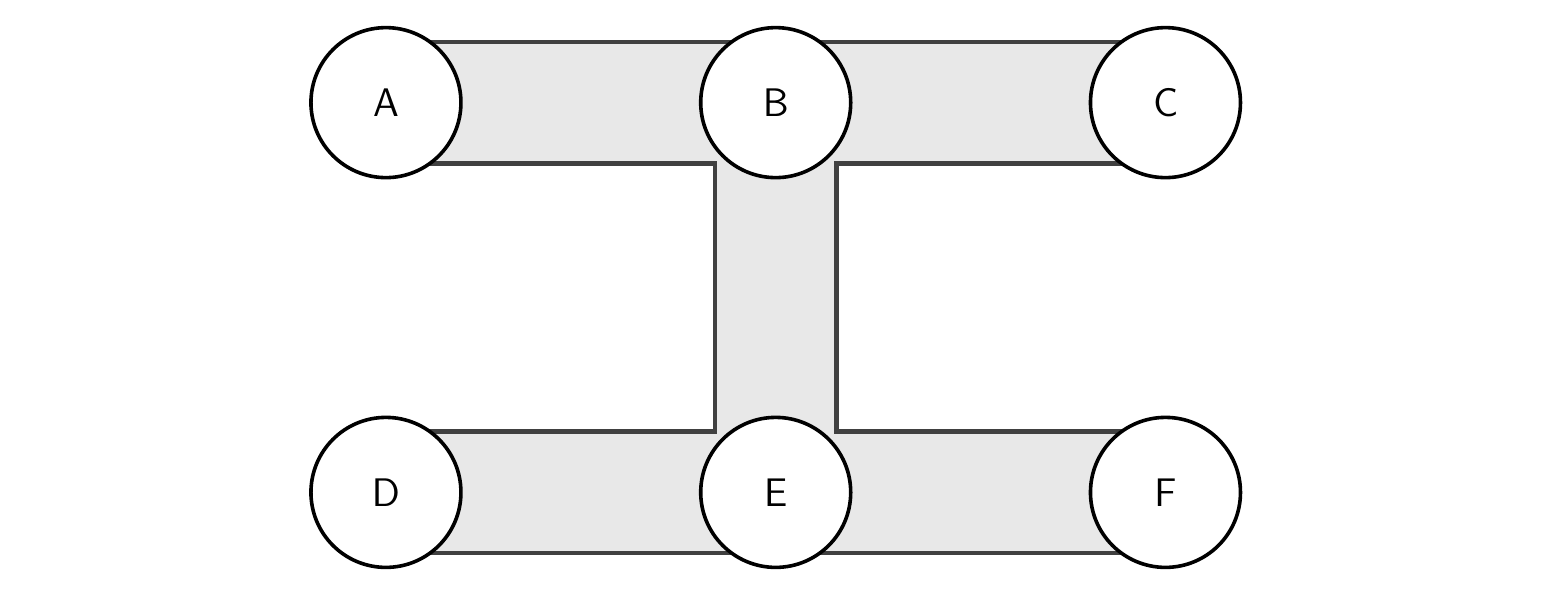
\begin{tikzpicture}
\useasboundingbox (0,0) rectangle (19.0,6.855);
\draw[bandout] (4.550,0.953) -- (9.500,0.953);
\draw[bandout] (9.500,0.953) -- (14.450,0.953);
\draw[bandout] (4.550,5.903) -- (9.500,5.903);
\draw[bandout] (9.500,5.903) -- (14.450,5.903);
\draw[bandout] (9.500,0.953) -- (9.500,5.903);
\draw[bandfill] (4.550,0.953) -- (9.500,0.953);
\draw[bandfill] (9.500,0.953) -- (14.450,0.953);
\draw[bandfill] (4.550,5.903) -- (9.500,5.903);
\draw[bandfill] (9.500,5.903) -- (14.450,5.903);
\draw[bandfill] (9.500,0.953) -- (9.500,5.903);
\draw[island] (4.550,0.953) circle (0.9525);
\node[islandlabel] at (4.550,0.953) {D};
\draw[island] (4.550,5.903) circle (0.9525);
\node[islandlabel] at (4.550,5.903) {A};
\draw[island] (9.500,0.953) circle (0.9525);
\node[islandlabel] at (9.500,0.953) {E};
\draw[island] (9.500,5.903) circle (0.9525);
\node[islandlabel] at (9.500,5.903) {B};
\draw[island] (14.450,0.953) circle (0.9525);
\node[islandlabel] at (14.450,0.953) {F};
\draw[island] (14.450,5.903) circle (0.9525);
\node[islandlabel] at (14.450,5.903) {C};
\end{tikzpicture}


\par\vspace{9mm}

\begin{minipage}{\linewidth}\raggedright
\prob{6}How can you tell, without walking, whether a town has a walk that picks up every counter, and where such a walk can start and end?

\vspace{5mm}\noindent \begin{tikzpicture}
\useasboundingbox (0,0) rectangle (19.0,6.000);
\draw[black!55, line width=0.6pt] (0.000,0.050) -- ++(19.0,0);
\draw[black!55, line width=0.6pt] (0.000,1.050) -- ++(19.0,0);
\draw[black!55, line width=0.6pt] (0.000,2.050) -- ++(19.0,0);
\draw[black!55, line width=0.6pt] (0.000,3.050) -- ++(19.0,0);
\draw[black!55, line width=0.6pt] (0.000,4.050) -- ++(19.0,0);
\draw[black!55, line width=0.6pt] (0.000,5.050) -- ++(19.0,0);
\end{tikzpicture}
\end{minipage}


\par\vspace{9mm}

\begin{minipage}{\linewidth}\raggedright
\prob{7}Trace each picture with a colored pencil, without lifting the pencil and without going over a line twice. If a picture cannot be traced this way, explain how you know.

\vspace{5mm}\noindent 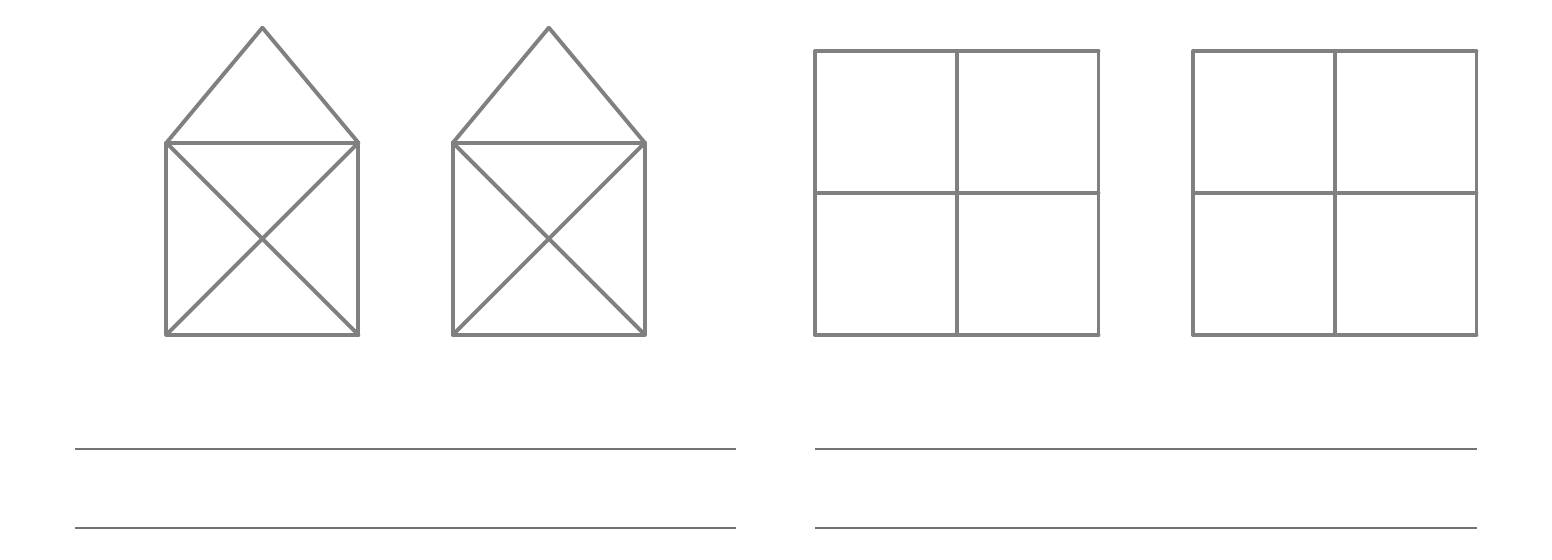
\begin{tikzpicture}
\useasboundingbox (0,0) rectangle (19.0,6.400);
\draw[stroke] (1.762,2.500) -- (4.200,2.500);
\draw[stroke] (4.200,2.500) -- (4.200,4.938);
\draw[stroke] (4.200,4.938) -- (1.762,4.938);
\draw[stroke] (1.762,4.938) -- (1.762,2.500);
\draw[stroke] (1.762,2.500) -- (4.200,4.938);
\draw[stroke] (4.200,2.500) -- (1.762,4.938);
\draw[stroke] (1.762,4.938) -- (2.981,6.400);
\draw[stroke] (2.981,6.400) -- (4.200,4.938);
\draw[stroke] (5.400,2.500) -- (7.837,2.500);
\draw[stroke] (7.837,2.500) -- (7.837,4.938);
\draw[stroke] (7.837,4.938) -- (5.400,4.938);
\draw[stroke] (5.400,4.938) -- (5.400,2.500);
\draw[stroke] (5.400,2.500) -- (7.837,4.938);
\draw[stroke] (7.837,2.500) -- (5.400,4.938);
\draw[stroke] (5.400,4.938) -- (6.619,6.400);
\draw[stroke] (6.619,6.400) -- (7.837,4.938);
\draw[black!55, line width=0.6pt] (0.600,0.050) -- ++(8.400,0);
\draw[black!55, line width=0.6pt] (0.600,1.050) -- ++(8.400,0);
\draw[stroke] (10.000,2.500) -- (13.600,2.500);
\draw[stroke] (13.600,2.500) -- (13.600,6.100);
\draw[stroke] (13.600,6.100) -- (10.000,6.100);
\draw[stroke] (10.000,6.100) -- (10.000,2.500);
\draw[stroke] (11.800,2.500) -- (11.800,6.100);
\draw[stroke] (10.000,4.300) -- (13.600,4.300);
\draw[stroke] (14.800,2.500) -- (18.400,2.500);
\draw[stroke] (18.400,2.500) -- (18.400,6.100);
\draw[stroke] (18.400,6.100) -- (14.800,6.100);
\draw[stroke] (14.800,6.100) -- (14.800,2.500);
\draw[stroke] (16.600,2.500) -- (16.600,6.100);
\draw[stroke] (14.800,4.300) -- (18.400,4.300);
\draw[black!55, line width=0.6pt] (10.000,0.050) -- ++(8.400,0);
\draw[black!55, line width=0.6pt] (10.000,1.050) -- ++(8.400,0);
\end{tikzpicture}
\end{minipage}


\par\vspace{7mm}\noindent 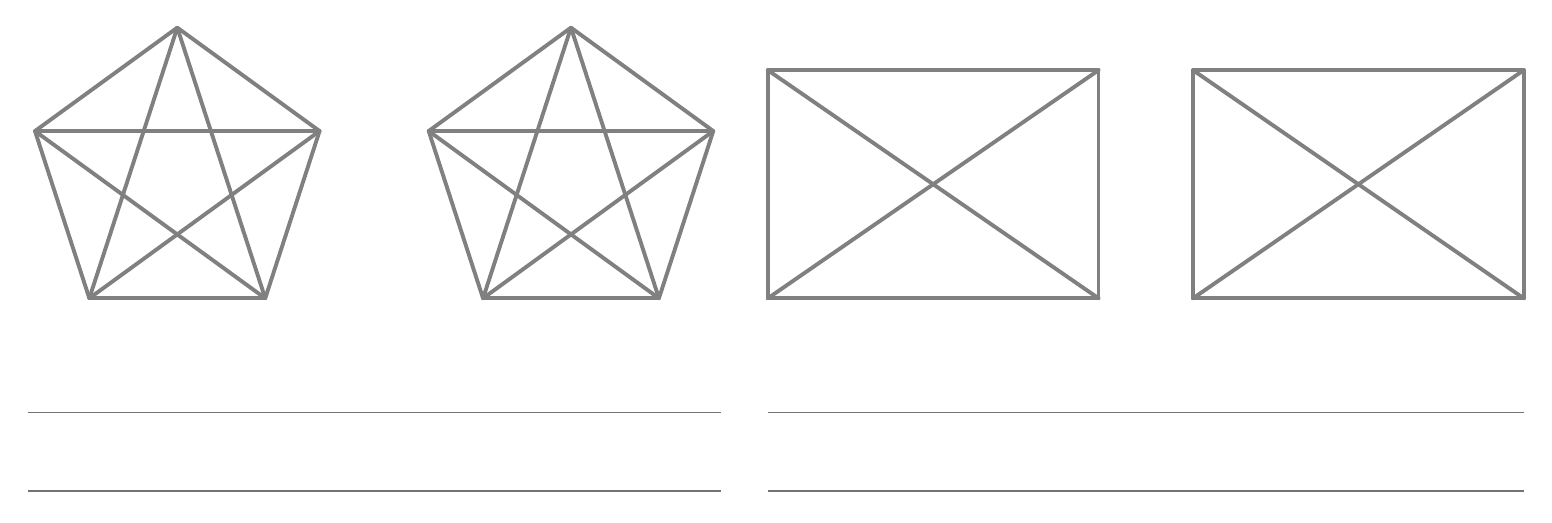
\begin{tikzpicture}
\useasboundingbox (0,0) rectangle (19.0,5.937);
\draw[stroke] (1.900,5.937) -- (0.093,4.624);
\draw[stroke] (0.093,4.624) -- (0.783,2.500);
\draw[stroke] (0.783,2.500) -- (3.017,2.500);
\draw[stroke] (3.017,2.500) -- (3.707,4.624);
\draw[stroke] (3.707,4.624) -- (1.900,5.937);
\draw[stroke] (1.900,5.937) -- (0.783,2.500);
\draw[stroke] (0.093,4.624) -- (3.017,2.500);
\draw[stroke] (0.783,2.500) -- (3.707,4.624);
\draw[stroke] (3.017,2.500) -- (1.900,5.937);
\draw[stroke] (3.707,4.624) -- (0.093,4.624);
\draw[stroke] (6.900,5.937) -- (5.093,4.624);
\draw[stroke] (5.093,4.624) -- (5.783,2.500);
\draw[stroke] (5.783,2.500) -- (8.017,2.500);
\draw[stroke] (8.017,2.500) -- (8.707,4.624);
\draw[stroke] (8.707,4.624) -- (6.900,5.937);
\draw[stroke] (6.900,5.937) -- (5.783,2.500);
\draw[stroke] (5.093,4.624) -- (8.017,2.500);
\draw[stroke] (5.783,2.500) -- (8.707,4.624);
\draw[stroke] (8.017,2.500) -- (6.900,5.937);
\draw[stroke] (8.707,4.624) -- (5.093,4.624);
\draw[black!55, line width=0.6pt] (0.000,0.050) -- ++(8.800,0);
\draw[black!55, line width=0.6pt] (0.000,1.050) -- ++(8.800,0);
\draw[stroke] (9.400,2.500) -- (13.600,2.500);
\draw[stroke] (13.600,2.500) -- (13.600,5.397);
\draw[stroke] (13.600,5.397) -- (9.400,5.397);
\draw[stroke] (9.400,5.397) -- (9.400,2.500);
\draw[stroke] (9.400,2.500) -- (13.600,5.397);
\draw[stroke] (13.600,2.500) -- (9.400,5.397);
\draw[stroke] (14.800,2.500) -- (19.000,2.500);
\draw[stroke] (19.000,2.500) -- (19.000,5.397);
\draw[stroke] (19.000,5.397) -- (14.800,5.397);
\draw[stroke] (14.800,5.397) -- (14.800,2.500);
\draw[stroke] (14.800,2.500) -- (19.000,5.397);
\draw[stroke] (19.000,2.500) -- (14.800,5.397);
\draw[black!55, line width=0.6pt] (9.400,0.050) -- ++(9.600,0);
\draw[black!55, line width=0.6pt] (9.400,1.050) -- ++(9.600,0);
\end{tikzpicture}


\par\vspace{7mm}\noindent 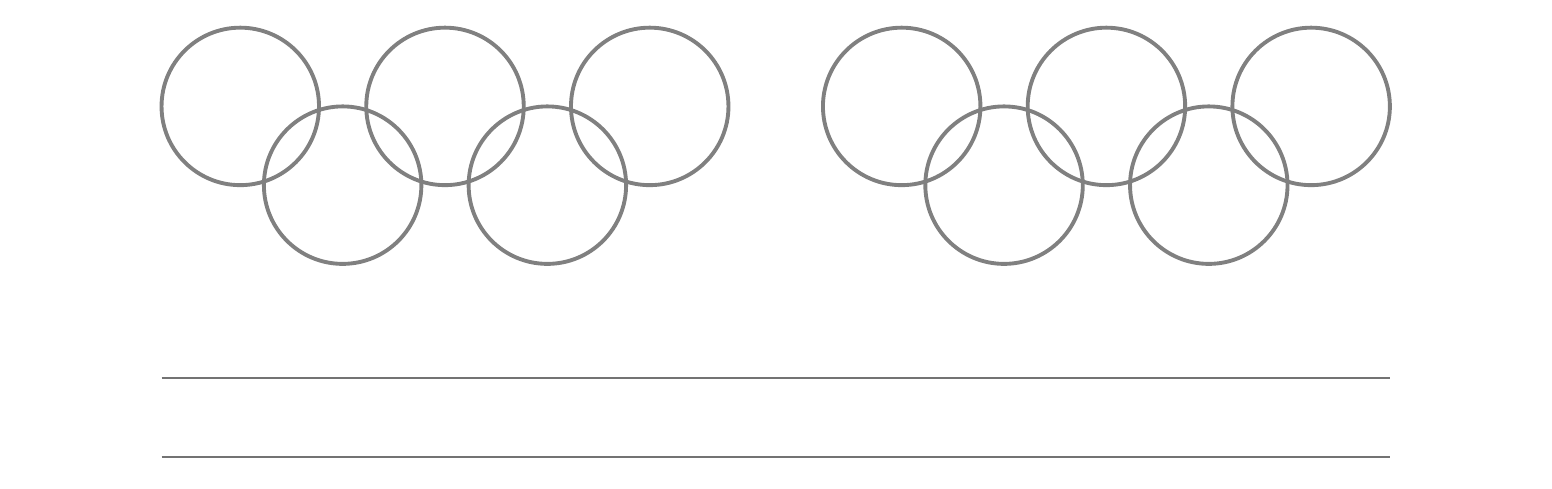
\begin{tikzpicture}
\useasboundingbox (0,0) rectangle (19.0,5.500);
\draw[stroke] (2.700,4.500) circle (1.000);
\draw[stroke] (5.300,4.500) circle (1.000);
\draw[stroke] (7.900,4.500) circle (1.000);
\draw[stroke] (4.000,3.500) circle (1.000);
\draw[stroke] (6.600,3.500) circle (1.000);
\draw[stroke] (11.100,4.500) circle (1.000);
\draw[stroke] (13.700,4.500) circle (1.000);
\draw[stroke] (16.300,4.500) circle (1.000);
\draw[stroke] (12.400,3.500) circle (1.000);
\draw[stroke] (15.000,3.500) circle (1.000);
\draw[black!55, line width=0.6pt] (1.700,0.050) -- ++(15.600,0);
\draw[black!55, line width=0.6pt] (1.700,1.050) -- ++(15.600,0);
\end{tikzpicture}


\par\vspace{7mm}\noindent 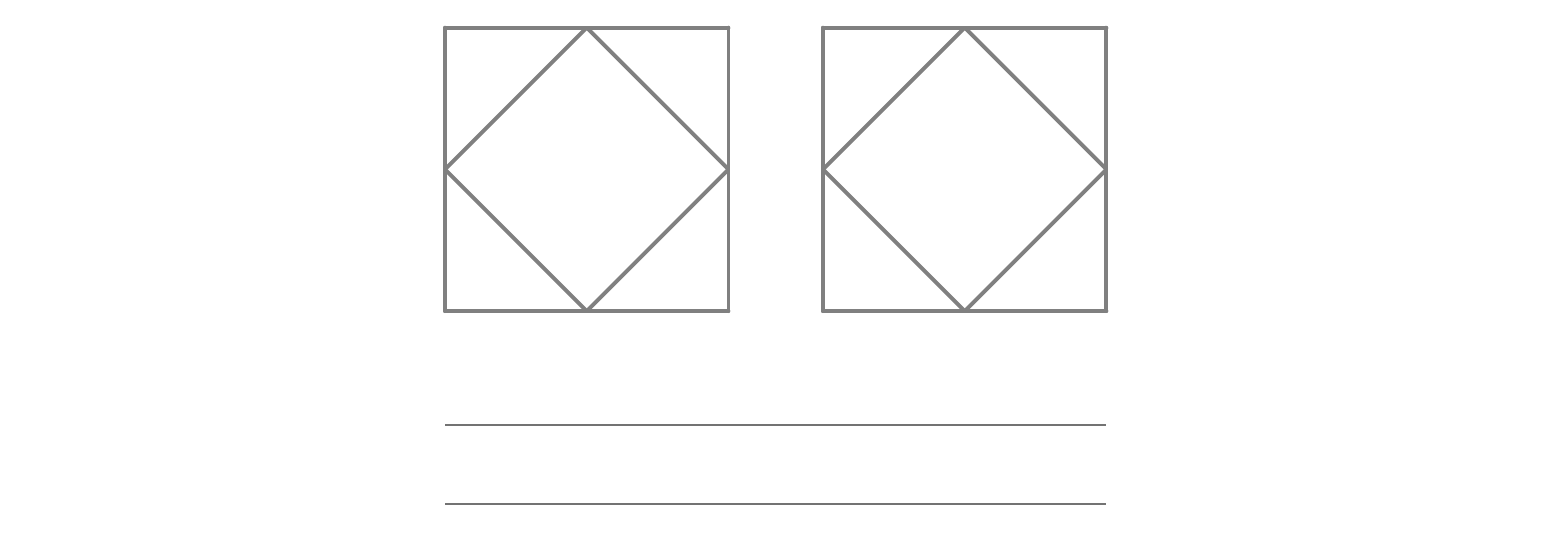
\begin{tikzpicture}
\useasboundingbox (0,0) rectangle (19.0,6.100);
\draw[stroke] (5.300,2.500) -- (8.900,2.500);
\draw[stroke] (8.900,2.500) -- (8.900,6.100);
\draw[stroke] (8.900,6.100) -- (5.300,6.100);
\draw[stroke] (5.300,6.100) -- (5.300,2.500);
\draw[stroke] (7.100,2.500) -- (8.900,4.300);
\draw[stroke] (8.900,4.300) -- (7.100,6.100);
\draw[stroke] (7.100,6.100) -- (5.300,4.300);
\draw[stroke] (5.300,4.300) -- (7.100,2.500);
\draw[stroke] (10.100,2.500) -- (13.700,2.500);
\draw[stroke] (13.700,2.500) -- (13.700,6.100);
\draw[stroke] (13.700,6.100) -- (10.100,6.100);
\draw[stroke] (10.100,6.100) -- (10.100,2.500);
\draw[stroke] (11.900,2.500) -- (13.700,4.300);
\draw[stroke] (13.700,4.300) -- (11.900,6.100);
\draw[stroke] (11.900,6.100) -- (10.100,4.300);
\draw[stroke] (10.100,4.300) -- (11.900,2.500);
\draw[black!55, line width=0.6pt] (5.300,0.050) -- ++(8.400,0);
\draw[black!55, line width=0.6pt] (5.300,1.050) -- ++(8.400,0);
\end{tikzpicture}


\par\vspace{9mm}

\begin{minipage}{\linewidth}\raggedright
\prob{8}Build each of these towns with hexagons and craft sticks for your partner to walk. Draw each town you build.

\vspace{5mm}\noindent \begin{tikzpicture}
\useasboundingbox (0,0) rectangle (19.0,9.400);
\draw[line width=0.9pt, black!70] (0.000,0.000) rectangle ++(9.0,8.0);
\node[anchor=north west, inner sep=0pt, text width=9.00cm, align=left] at (0.000,9.400) {4 islands and 6 bridges. A walk that picks up every counter can start on any island.};
\draw[line width=0.9pt, black!70] (10.000,0.000) rectangle ++(9.0,8.0);
\node[anchor=north west, inner sep=0pt, text width=9.00cm, align=left] at (10.000,9.400) {5 islands and 5 bridges. No walk picks up every counter.};
\end{tikzpicture}
\end{minipage}


\par\vspace{7mm}\noindent \begin{tikzpicture}
\useasboundingbox (0,0) rectangle (19.0,9.400);
\draw[line width=0.9pt, black!70] (0.000,0.000) rectangle ++(9.0,8.0);
\node[anchor=north west, inner sep=0pt, text width=9.00cm, align=left] at (0.000,9.400) {6 islands and 8 bridges. A walk that picks up every counter can start only on A or on F.};
\draw[line width=0.9pt, black!70] (10.000,0.000) rectangle ++(9.0,8.0);
\node[anchor=north west, inner sep=0pt, text width=9.00cm, align=left] at (10.000,9.400) {3 islands and 5 bridges. A walk that picks up every counter can start only on A or on B.};
\end{tikzpicture}


\par\vspace{9mm}

\begin{minipage}{\linewidth}\raggedright
\prob{9}Can you make a town with at least one bridge where a walk that picks up every counter can start on only one island? Make one, or explain why it cannot be done.

\vspace{5mm}\noindent \begin{tikzpicture}
\useasboundingbox (0,0) rectangle (19.0,10.000);
\draw[black!55, line width=0.6pt] (0.000,0.050) -- ++(10.0,0);
\draw[black!55, line width=0.6pt] (0.000,1.050) -- ++(10.0,0);
\draw[black!55, line width=0.6pt] (0.000,2.050) -- ++(10.0,0);
\draw[black!55, line width=0.6pt] (0.000,3.050) -- ++(10.0,0);
\draw[black!55, line width=0.6pt] (0.000,4.050) -- ++(10.0,0);
\draw[black!55, line width=0.6pt] (0.000,5.050) -- ++(10.0,0);
\draw[black!55, line width=0.6pt] (0.000,6.050) -- ++(10.0,0);
\draw[black!55, line width=0.6pt] (0.000,7.050) -- ++(10.0,0);
\draw[black!55, line width=0.6pt] (0.000,8.050) -- ++(10.0,0);
\draw[black!55, line width=0.6pt] (0.000,9.050) -- ++(10.0,0);
\draw[line width=0.9pt, black!70] (11.000,0.000) rectangle ++(8.0,10.0);
\end{tikzpicture}
\end{minipage}


\par\vspace{9mm}

\newpage

\begin{minipage}{\linewidth}\raggedright
\prob{10}A bridge can hold two counters, and then a walk can cross it two times. In each town, put a second counter on as few bridges as you can so that a walk can pick up every counter and end on the island where it started. Color each bridge that gets a second counter.

\vspace{5mm}\noindent 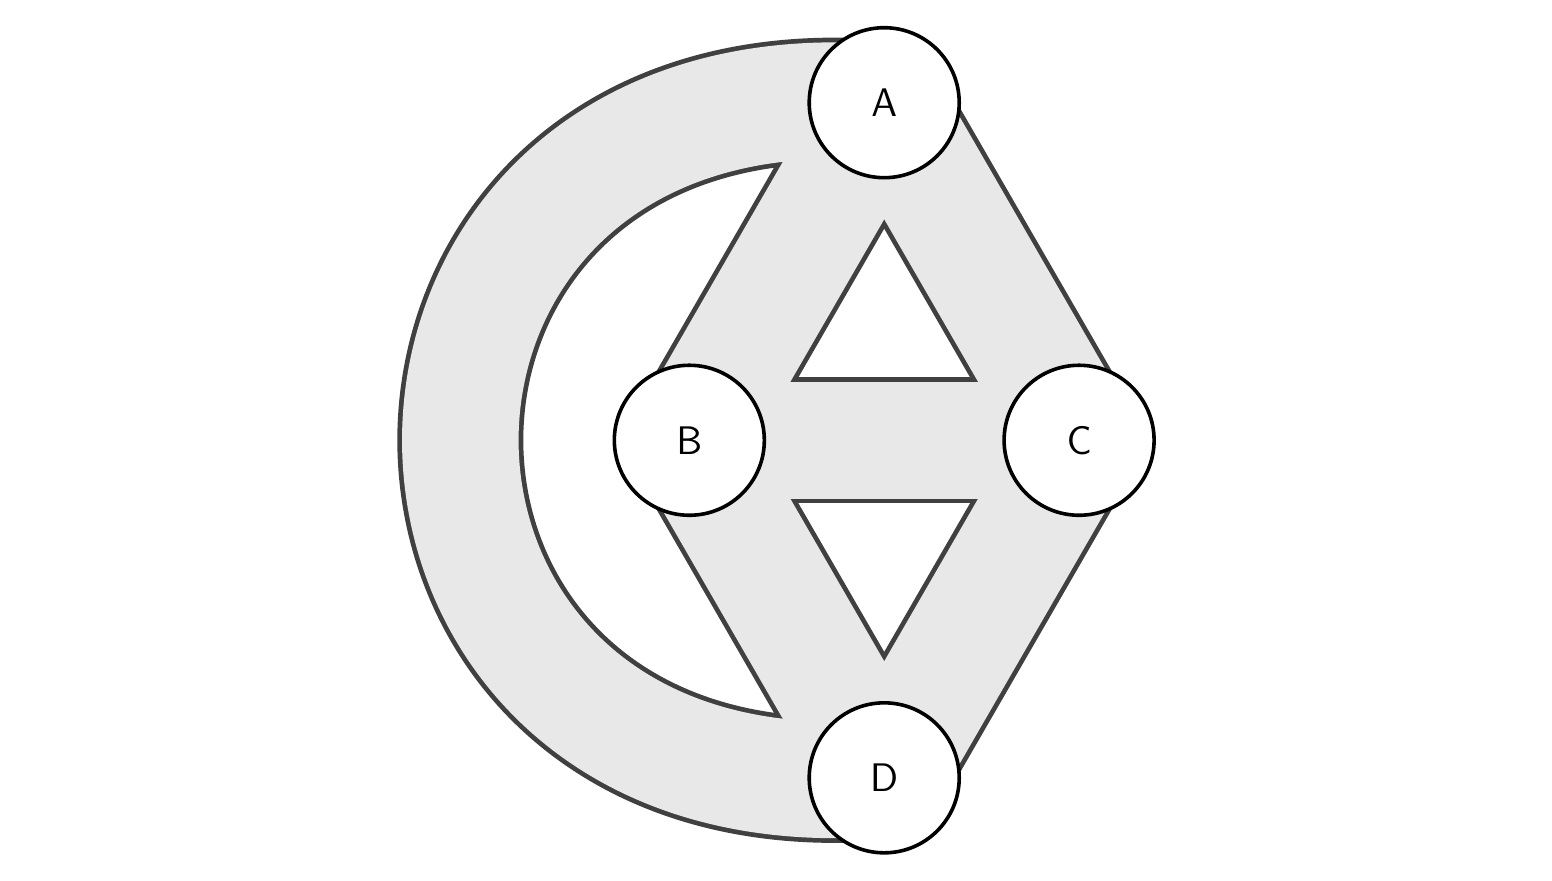
\begin{tikzpicture}
\useasboundingbox (0,0) rectangle (19.0,10.479);
\draw[bandout] (8.403,5.239) -- (13.353,5.239);
\draw[bandout] (8.403,5.239) -- (10.878,0.952);
\draw[bandout] (8.403,5.239) -- (10.878,9.526);
\draw[bandout] (13.353,5.239) -- (10.878,0.952);
\draw[bandout] (13.353,5.239) -- (10.878,9.526);
\draw[bandout] (10.878,0.952) .. controls (3.700,0.353) and (3.700,10.126) .. (10.878,9.526);
\draw[bandfill] (8.403,5.239) -- (13.353,5.239);
\draw[bandfill] (8.403,5.239) -- (10.878,0.952);
\draw[bandfill] (8.403,5.239) -- (10.878,9.526);
\draw[bandfill] (13.353,5.239) -- (10.878,0.952);
\draw[bandfill] (13.353,5.239) -- (10.878,9.526);
\draw[bandfill] (10.878,0.952) .. controls (3.700,0.353) and (3.700,10.126) .. (10.878,9.526);
\draw[island] (8.403,5.239) circle (0.9525);
\node[islandlabel] at (8.403,5.239) {B};
\draw[island] (13.353,5.239) circle (0.9525);
\node[islandlabel] at (13.353,5.239) {C};
\draw[island] (10.878,0.952) circle (0.9525);
\node[islandlabel] at (10.878,0.952) {D};
\draw[island] (10.878,9.526) circle (0.9525);
\node[islandlabel] at (10.878,9.526) {A};
\end{tikzpicture}
\end{minipage}


\par\vspace{7mm}\noindent 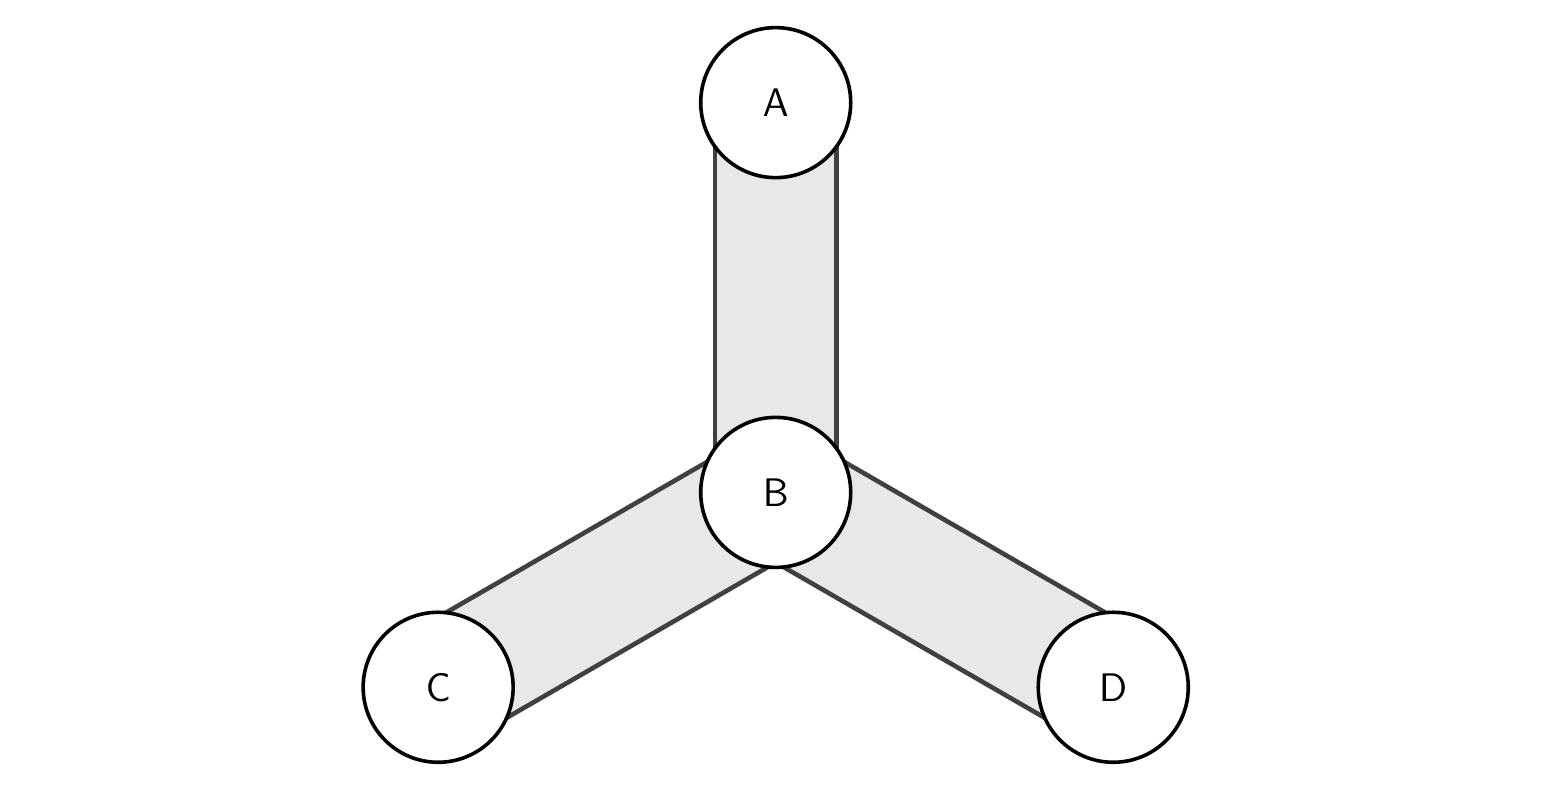
\begin{tikzpicture}
\useasboundingbox (0,0) rectangle (19.0,9.330);
\draw[bandout] (9.500,3.428) -- (9.500,8.378);
\draw[bandout] (9.500,3.428) -- (5.213,0.953);
\draw[bandout] (9.500,3.428) -- (13.787,0.953);
\draw[bandfill] (9.500,3.428) -- (9.500,8.378);
\draw[bandfill] (9.500,3.428) -- (5.213,0.953);
\draw[bandfill] (9.500,3.428) -- (13.787,0.953);
\draw[island] (9.500,3.428) circle (0.9525);
\node[islandlabel] at (9.500,3.428) {B};
\draw[island] (9.500,8.378) circle (0.9525);
\node[islandlabel] at (9.500,8.378) {A};
\draw[island] (5.213,0.953) circle (0.9525);
\node[islandlabel] at (5.213,0.953) {C};
\draw[island] (13.787,0.953) circle (0.9525);
\node[islandlabel] at (13.787,0.953) {D};
\end{tikzpicture}


\par\vspace{9mm}
\end{document}
